\documentclass[a4paper,12pt]{article}
\usepackage[utf8]{inputenc}
\usepackage[T1]{fontenc}
\usepackage[italian]{babel}
\usepackage[sfdefault]{atkinson}
\renewcommand*\familydefault{\sfdefault}
\usepackage{float}
\usepackage{microtype}
\usepackage{geometry}
\usepackage{setspace}
\usepackage{enumitem}
\usepackage{titlesec}
\usepackage{chngpage}
\usepackage{tocloft}
\usepackage{longtable}
\usepackage{ltablex}
\usepackage{array}
\usepackage{graphicx}
\usepackage{fancyhdr}
\usepackage[table]{xcolor}
\usepackage{color,soul}
\usepackage[most]{tcolorbox}
\usepackage{nameref}
\usepackage[colorlinks=true]{hyperref}

\usepackage{titlesec}
\setlength{\parindent}{0pt}

\setcounter{tocdepth}{4} 
\setcounter{tocdepth}{5}

\setcounter{secnumdepth}{5}


\hypersetup{
    linkcolor=black,
    urlcolor=blue
}

\definecolor{lightblack}{gray}{0.35}
\newcommand{\glossario}[1]{\textit{#1}\textsubscript{\textbf{\textit{\textcolor{lightblack}{G}}}}}
\newcommand{\ped}[1]{\textsubscript{#1}}

\pagestyle{fancy}
\setlength{\headwidth}{\textwidth}
\fancyhfoffset[L,R]{0pt}
\lhead{\rightmark}
\rhead{7-ZPUs}
\lfoot{Norme di Progetto}
\rfoot{\thepage}
\cfoot{}
\renewcommand{\headrulewidth}{0.8pt}
\renewcommand{\footrulewidth}{0.8pt}

\renewcommand{\contentsname}{Indice}
\renewcommand{\listfigurename}{Indice delle immagini}
\renewcommand{\listtablename}{Indice delle tabelle}

% Configurazione per rendere le metriche ben visibili
\newcommand{\metricdef}[3]{
    \subsubsection*{#1 - #2}
    \textbf{Descrizione:} #3
}

\newcommand{\metricformula}[1]{
    \\[0.5em]
    \textbf{Formula di calcolo:}
    \begin{equation*}
        #1
    \end{equation*}
}


\geometry{margin=2.5cm}
\setstretch{1.1}

\titleformat{\section}{\Large\bfseries}{\thesection}{1em}{}
\titleformat{\subsection}{\large\bfseries}{\thesubsection}{1em}{}
\titleformat{\subsubsection}{\normalsize\bfseries}{\thesubsubsection}{1em}{}
\titleformat{\paragraph}{\normalsize\bfseries}{\theparagraph}{1em}{}
\titleformat{\subparagraph}{\normalsize\bfseries}{\thesubparagraph}{1em}{}


\titlespacing*{\paragraph}
{0pt}{3.25ex plus 1ex minus .2ex}{1.5ex plus .2ex}

\begin{document}

\begin{center}
    \includegraphics[width=9.5cm]{../../assets/logo7ZPUs.jpg}\\
    \small\hspace{10cm} 7zpus.swe@gmail.com\\
    \vspace{0.5cm}
    \LARGE \textbf{Norme di Progetto}\\
    \vspace{0.3cm}
    \normalsize \textbf{Versione:} 1.0.0\\
    \textbf{Responsabile:} Laoud Zakaria \\
    \textbf{Destinatari:} Sanmarco Informatica S.p.A., Prof. Tullio Vardanega, Prof. Riccardo Cardin, Team 7-ZPUs \\
\end{center}

\vspace{0.3cm}
\hrule
\vspace{0.5cm}

\section*{Tabella di Versionamento}
\setlength{\LTleft}{-0.8cm}

\begin{spacing}{1.1}
    \begin{longtable}{|c|c|p{3.2cm}|p{3.2cm}|p{5cm}|}
        \hline
        \textbf{Versione} & \textbf{Data} & \textbf{Autore}  & \textbf{Verificatore} & \textbf{Descrizione} \\
        \hline
        1.0.1             & 2026/03/17    & Laoud Zakaria    & Soligo Lorenzo        & Stesura paragrafo sulla progettazione \\
        \hline
        1.0.0             & 2026/02/24    & Laoud Zakaria    & Soligo Lorenzo        & Approvazione per baseline RTB \\
        \hline
        0.14              & 2026/02/11    & Vigolo Davide    & Soligo Lorenzo        & Definizione metriche di qualità                                                                                                          \\
        \hline
        0.13              & 2026/02/09    & Fattoni Antonio  & Vigolo Davide         & Correzione processo di documentazione e controllo della configurazione                                                                   \\
        \hline
        0.12              & 2026/02/08    & Vigolo Davide    & Soligo Lorenzo        & Definizione metriche di qualità                                                                                                          \\
        \hline
        0.11              & 2026/02/06    & Laoud Zakaria    & Soligo Lorenzo        & Stesura paragrafi 3.6, 3.7, 3.8                                                                                                          \\
        \hline
        0.10              & 2025/01/25    & Aaron Gingillino & Georgescu Diana       & Scrittura paragrafi 2.2, 4.1                                                                                                             \\
        \hline
        0.9               & 2025/01/25    & Aaron Gingillino & Fattoni Antonio       & Scrittura paragrafi 3.3, 3.4                                                                                                             \\
        \hline
        0.8.1             & 2026/01/19    & Soligo Lorenzo   & Laoud Zakaria         & Fine scrittura paragrafi 4.2, 4.3, 4.4                                                                                                   \\
        \hline
        0.8               & 2026/01/11    & Soligo Lorenzo   & Laoud Zakaria         & Stesura paragrafi 4.2, 4.3, 4.4                                                                                                          \\
        \hline
        0.7               & 2025/12/15    & Rocco Matteo A.  & Georgescu Diana       & Stesura paragrafo 5                                                                                                                      \\
        \hline
        0.6               & 2025/12/10    & Georgescu Diana  & Soligo Lorenzo        & Stesura sottosezioni 2.3, 2.4                                                                                                            \\
        \hline
        0.5               & 2025/12/01    & Soligo Lorenzo   & Rocco Matteo A.       & Aggiornamento nuovo standard per gestione branch, convenzioni sui nomi, date e versioni. Sezioni 3.1.2, 3.3, 3.2.1.1.1, 3.2.4, 4.2.3.2.1 \\
        \hline
        0.4.1             & 2025/11/28    & Soligo Lorenzo   & Fattoni Antonio       & Correzione nella Procedura di Revisione Paragrafo 3.1.3.1 e aggiornamento immagini                                                       \\
        \hline
        0.4               & 2025/11/26    & Soligo Lorenzo   & Fattoni Antonio       & Ristrutturazione completa Processi (ISO 12207: Attività-Procedure-Strumenti)                                                             \\
        \hline
        0.3               & 2025/11/25    & Soligo Lorenzo   & Fattoni Antonio       & Creazione e stesura sezioni Processi di Infrastruttura e sottosezioni 4.2.1-4.3. Nuova struttura Paragrafi sottoParagrafi                \\
        \hline
        0.2               & 2025/11/22    & Soligo Lorenzo   & Fattoni Antonio       & Creazione e stesura sezioni Documentazione e sottosezioni 3.1-3.1.5                                                                      \\
        \hline
        0.1               & 2025/11/16    & Rocco Matteo A.  & Soligo Lorenzo        & Creazione e stesura sezioni Introduzione e Processo di fornitura                                                                         \\
        \hline
    \end{longtable}
\end{spacing}
\newpage

\tableofcontents
\listoffigures

\section{Introduzione}

\subsection{Scopo}
Questo documento ha l'obiettivo di definire e normare il \glossario{Way of
    Working}, ovvero le regole di lavoro che ogni membro del gruppo deve rispettare
durante lo svolgimento delle \glossario{attività di progetto} volte allo
sviluppo dell'applicativo software \glossario{\textbf{DIPReader}}, proposto
dall'azienda Sanmarco Informatica. A ciascun membro è richiesto di seguirle
integralmente per poter lavorare in maniera efficace, efficiente e omogenea.
Data la natura incrementale della redazione del documento, il
\glossario{responsabile} di progetto ha il compito di mantenere aggiornate le
presenti norme e gli eventuali riferimenti ad altri documenti in esse
contenuti.
\subsection{Glossario}
Ogni termine tecnico o con un significato particolare nell'ambito
dell'\glossario{Ingegneria del Software}, utilizzato nella documentazione di
progetto, è definito nell'apposito documento
\href{https://7-zpus.github.io/Docs/assets/2_RTB/DocumentiInterni/Glossario.pdf}{\ul{Glossario
        1.0}\setulcolor{black}}\ped{(v1.0.0)}.
\subsection{Riferimenti}
Il gruppo ha redatto il presente documento in conformità con lo Standard
ISO/IEC 12207:1995, integrandolo occasionalmente con approfondimenti tratti
dalla sua versione più recente, ISO/IEC/IEEE 12207:2017, per includere dettagli
aggiuntivi sugli approcci \glossario{\textit{Agile}} e iterativi che
caratterizzano lo sviluppo \glossario{software} moderno.
\subsubsection{Riferimenti Normativi}
\begin{itemize}
    \item \href{https://www.math.unipd.it/~tullio/IS-1/2009/Approfondimenti/ISO_12207-1995.pdf}{\ul{Standard ISO/IEC 12207:1995}\setulcolor{black}} \ped{(ultimo accesso: 20/02/2026)}
    \item \href{https://www.iso.org/standard/63712.html}{\ul{Standard ISO/IEC/IEEE 12207:2017}} \ped{(ultimo accesso: 20/02/2026)}
    \item \href{https://www.iso.org/standard/71952.html}{\ul{Standard ISO/IEC/IEEE 24765:2017}} \ped{(ultimo accesso: 20/02/2026)}
    \item \href{https://www.math.unipd.it/~tullio/IS-1/2025/Progetto/C3.pdf}{\ul{Capitolato C3: DIPReader}\setulcolor{black}} \ped{(ultimo accesso: 10/02/2026)}
    \item \href{https://www.math.unipd.it/~tullio/IS-1/2025/Dispense/PD1.pdf}{\ul{Regolamento di Progetto Didattico a.a.
                  2025/2026}\setulcolor{black}} \ped{(ultimo accesso: 20/02/2026)}
\end{itemize}

\subsubsection{Riferimenti Informativi}
\begin{itemize}
    \item Dispense del corso di Ingegneria del Software 2025/2026:
          \begin{itemize}
              \item \href{https://www.math.unipd.it/~tullio/IS-1/2025/Dispense/T01.pdf}{\ul{https://www.math.unipd.it/~tullio/IS-1/2025/Dispense/T01.pdf}\setulcolor{black}} \ped{(ultimo accesso: 20/02/2026)}
              \item \href{https://www.math.unipd.it/~tullio/IS-1/2025/Dispense/T02.pdf}{\ul{https://www.math.unipd.it/~tullio/IS-1/2025/Dispense/T02.pdf}\setulcolor{black}} \ped{(ultimo accesso: 20/02/2026)}
              \item \href{https://www.math.unipd.it/~tullio/IS-1/2025/Dispense/T03.pdf}{\ul{https://www.math.unipd.it/~tullio/IS-1/2025/Dispense/T03.pdf}\setulcolor{black}} \ped{(ultimo accesso: 20/02/2026)}
              \item \href{https://www.math.unipd.it/~tullio/IS-1/2025/Dispense/T04.pdf}{\ul{https://www.math.unipd.it/~tullio/IS-1/2025/Dispense/T04.pdf}\setulcolor{black}} \ped{(ultimo accesso: 20/02/2026)}
              \item \href{https://www.math.unipd.it/~tullio/IS-1/2025/Dispense/T05.pdf}{\ul{https://www.math.unipd.it/~tullio/IS-1/2025/Dispense/T05.pdf}\setulcolor{black}} \ped{(ultimo accesso: 20/02/2026)}
              \item \href{https://www.math.unipd.it/~tullio/IS-1/2025/Dispense/T06.pdf}{\ul{https://www.math.unipd.it/~tullio/IS-1/2025/Dispense/T06.pdf}\setulcolor{black}} \ped{(ultimo accesso: 20/02/2026)}
              \item \href{https://www.math.unipd.it/~tullio/IS-1/2025/Dispense/T07.pdf}{\ul{https://www.math.unipd.it/~tullio/IS-1/2025/Dispense/T07.pdf}\setulcolor{black}} \ped{(ultimo accesso: 20/02/2026)}
              \item \href{https://www.math.unipd.it/~tullio/IS-1/2025/Dispense/T08.pdf}{\ul{https://www.math.unipd.it/~tullio/IS-1/2025/Dispense/T08.pdf}\setulcolor{black}} \ped{(ultimo accesso: 17/02/2025)}
              \item \href{https://www.math.unipd.it/~tullio/IS-1/2025/Dispense/T09.pdf}{\ul{https://www.math.unipd.it/~tullio/IS-1/2025/Dispense/T09.pdf}\setulcolor{black}} \ped{(ultimo accesso: 17/02/2025)}
              \item \href{https://www.math.unipd.it/~tullio/IS-1/2025/Dispense/T10.pdf}{\ul{https://www.math.unipd.it/~tullio/IS-1/2025/Dispense/T10.pdf}\setulcolor{black}} \ped{(ultimo accesso: 17/02/2025)}
              \item \href{https://www.math.unipd.it/~tullio/IS-1/2025/Dispense/T11.pdf}{\ul{https://www.math.unipd.it/~tullio/IS-1/2025/Dispense/T11.pdf}\setulcolor{black}} \ped{(ultimo accesso: 17/02/2025)}
          \end{itemize}
    \item \href{https://www.agid.gov.it/it/sicurezza/cert-pa/linee-guida-sviluppo-del-software-sicuro}{\ul{Linee Guida Sviluppo Sicuro AGID (Agenzia per l'Italia Digitale)}\setulcolor{black}} \ped{(ultimo accesso: 22/12/2026)}
    \item  \href{https://www.agid.gov.it/it/linee-guida#index-3}{\ul{Linee Guida sulla formazione, gestione e conservazione dei documenti informatici AGID}\setulcolor{black}} \ped{(ultimo accesso: 22/12/2026)}
    \item \href{https://www.lorenzopantieri.net/LaTeX_files/LaTeXpedia.pdf}{\ul{Documentazione \LaTeX{} by Lorenzo Pantieri}\setulcolor{black}} \ped{(ultimo accesso: 17/11/2025)}
    \item \href{https://confluence.atlassian.com/jira}{\ul{Documentazione Jira}\setulcolor{black}} \ped{(ultimo accesso: 20/02/2026)}
\end{itemize}

\section{Processi Primari}

\subsection{Processo di Fornitura}\label{processoDiFornitura}
Il \glossario{processo} di fornitura contiene le attività e i compiti svolti
dal \glossario{fornitore}. Questo processo è necessario per la comprensione dei
\glossario{requisiti} del prodotto da sviluppare. Per implementare
correttamente il processo il gruppo si impegna a svolgere le seguenti attività.

\subsubsection{Attività: Avvio}
Il fornitore analizza i requisiti necessari alla proposta di fornitura, tenendo
in considerazione eventuali vincoli organizzativi e normativi.

\paragraph{Procedura: analisi approfondita del capitolato di progetto}
Il fornitore deve estrarre i requisiti specificati dalla proponente,
identificando le funzionalità richieste, i vincoli tecnici e le aspettative di
qualità. Questa attività è condotta da tutti i membri del gruppo, al fine di
ottenere una analisi completa e condivisa del documento. Le considerazioni
fatte confluiscono nel documento di
\href{https://7-zpus.github.io/Docs/assets/1_Candidatura/AnalisiCapitolati.pdf}{\ul{Analisi
        dei capitolati}\setulcolor{black}} \ped{(v1.0.0)}
(§\ref{analisiDeiCapitolati}). I punti da analizzare sono i seguenti:
\begin{itemize}
    \item \textbf{Obiettivo}: identificare l'obiettivo di massima del progetto e le funzionalità richieste.
    \item \textbf{Dominio applicativo}: contesto di operatività del software nonché il target di utenti a cui è rivolto.
    \item \textbf{Dominio tecnico}: contesto tecnologico sul quale il software dovrà eventualmente integrarsi, vengono riportati i vincoli tecnologici.
    \item \textbf{Aspetti positivi}: identificare le opportunità formative e di crescita che il progetto può offrire, nonché i punti di forza del capitolato.
    \item \textbf{Aspetti negativi}: identificare le criticità e le sfide che il progetto può presentare, nonché i punti di debolezza del capitolato.
    \item \textbf{Possibili rischi}: identificare i rischi potenziali associati al progetto, come ad esempio la complessità tecnica, la mancanza di competenze specifiche o eventuali vincoli di tempo.
\end{itemize}
\paragraph{Strumenti}
\begin{itemize}
    \item \textbf{Discord:} strumento per la comunicazione asincrona e sincrona remota tra i membri del gruppo, sia essa vocale (sincrona) o testuale(asincrona).
    \item \textbf{\LaTeX}: per la redazione del documento di Analisi dei Capitolati.
\end{itemize}

\subsubsection{Attività: Preparazione della proposta di fornitura}\label{preparazionePropostaFornitura}
Il fornitore prepara la proposta di fornitura in risposta alle richieste della
proponente e definisce i termini in cui si articola la proposta.

\paragraph{Procedura: Valutazione delle risorse}
Il fornitore deve valutare i ruoli, i costi e le risorse disponibili per
soddisfare i requisiti di fornitura. Nello specifico:
\begin{itemize}
    \item \textbf{Ruoli necessari}: identificare i ruoli necessari per lo sviluppo del progetto, come ad esempio sviluppatori, verificatori, analisti, ecc.
    \item \textbf{Costi orari}: definire i costi orari per ciascun ruolo, tenendo conto delle competenze richieste e del mercato di riferimento.
    \item \textbf{Stima oraria per ruolo}: per ciascun ruolo stabilito, definire una stima oraria necessaria al completamento del progetto. Questa stima deve basarsi sui risultati dell'analisi del capitolato, e fungerà da limite di spesa non superabile.
    \item \textbf{Componenti del gruppo di progetto}: identificare i membri del gruppo di progetto.
    \item \textbf{Data di consegna stimata}: definire una data di consegna stimata per il completamento del progetto tenendo conto delle risorse stanziate nei punti precedenti.
\end{itemize}
queste valutazioni confluiscono nel documento \href{https://7-zpus.github.io/Docs/assets/1_Candidatura/PreventivoCostiEAssunzioneImpegni.pdf}{Preventivo costi e assunzione impegni}\setulcolor{black} \ped{(v1.0.0)} (§\ref{preventivoCostiEAssunzioneImpegni}).
\paragraph{Strumenti}
\begin{itemize}
    \item \textbf{Discord}: strumento per la comunicazione asincrona e sincrona remota tra i membri del gruppo, sia essa vocale (sincrona) o testuale(asincrona).
    \item \textbf{\LaTeX}: per la redazione del documento di Preventivo costi e assunzione impegni.
    \item \textbf{Foglio di calcolo}: per agevolare i calcoli e produrre le tabelle necessarie con facilità e garantendo correttezza.
\end{itemize}
\subsubsection{Attività: Accordo}
\glossario{Proponente} e fornitore entrano nella fase di definizione dell'accordo di
fornitura del prodotto software, prevedendo possibilità di negoziazione della
fornitura da parte del fornitore.

\paragraph{Procedura: ridefinizione dell'accordo di fornitura}
Il fornitore si adopera per ridefinire la proposta di fornitura, adattandola
alle esigenze della proponente, se possibile. Viene iterata nuovamente
l'attività di preparazione della proposta di fornitura
(§\ref{preparazionePropostaFornitura})

\paragraph{Strumenti}
\begin{itemize}
    \item \textbf{\LaTeX}: per la redazione del documento di ridefinizione dell'accordo di fornitura.
\end{itemize}

\subsubsection{Attività: Pianificazione}
si pianificano le attività necessarie per soddisfare i requisiti del cliente,
stabilendo tempi, risorse e costi. Viene definito il modello di sviluppo più
adatto al progetto, tenendo conto delle caratteristiche del progetto e delle
esigenze della proponente. E' inoltre fondamentale identificare potenziali
rischi che possono insorgere nello svolgimento.

\paragraph{Procedura: pianificazione delle attività}
Il fornitore deve pianificare il lavoro a lungo termine definendo milestone e
obiettivi intermedi.
%qui come definire una milestone (guida concreta)
In particolare l'identificazione delle milestone deve essere effettuata tenendo conto dei seguenti aspetti:
\begin{itemize}
    \item \textbf{Obiettivi di progetto}: identificare gli obiettivi principali del progetto e suddividerli in obiettivi intermedi, che rappresentano le milestone.
    \item \textbf{Tempi di consegna}: stabilire i tempi di consegna per ciascuna milestone, tenendo conto delle risorse disponibili e delle esigenze della proponente.
    \item \textbf{Risorse necessarie}: identificare le risorse necessarie per raggiungere ciascuna milestone, come ad esempio competenze specifiche, strumenti o infrastrutture.
    \item \textbf{Criteri di accettazione}: definire i criteri di accettazione per ciascuna milestone, in modo da garantire che il lavoro svolto soddisfi le aspettative della proponente.
    \item \textbf{Dipendenze tra le attività}: identificare eventuali dipendenze tra le attività necessarie per raggiungere le milestone, in modo da pianificare il lavoro in modo efficiente e evitare ritardi.
\end{itemize}
 La definizione poi risulta più efficiente se programmata a ritroso a partire dalla data di consegna stimata e dalle necessità del team (date di laurea, per esempio). Avendo un limite temporale facilita la definizione delle attività da svolgere al fine di raggiungere le milestone nelle finestre temporali stabilite.
Contemporaneamente con lo svolgersi del progetto, è necessario pianificare a
breve termine i periodi, definendo le attività da svolgere (vedi
§\ref{gestione_processi_organizzativi}).

\paragraph{Procedura: identificazione dei rischi}
Il fornitore deve valutare i potenziali \glossario{rischi} che potrebbero
insorgere durante lo sviluppo del prodotto e definire strategie di mitigazione
per affrontarli efficacemente. Vanno riportati, una volta individuati, nella
sezione apposita del documento Piano di Progetto (§\ref{pianoDiProgetto}). Per
ogni rischio si identificano le seguenti caratteristiche:
\begin{itemize}
    \item \textbf{Probabilità di occorrenza}: probabilità espressa in percentuale che il rischio si verifichi durante lo svolgimento del progetto.
    \item \textbf{Effetti}: intesi come grado di impatto sullo svolgersi del progetto
    \item \textbf{Descrizione}: descrizione del rischio
    \item \textbf{Strategia di mitigazione}: descrizione delle azioni da intraprendere per mitigare il rischio, qualora si verificasse.
    \item \textbf{Indicatori}: definizione di indicatori che permettano di identificare tempestivamente l'insorgere del rischio, in modo da poter attivare le strategie di mitigazione in tempo utile.
\end{itemize}
ogni rischio deve seguire la seguente nomenclatura:
\begin{center}
    \texttt{R[T][C]}
\end{center}
dove:
\begin{itemize}
    \item \textbf{T}: tipologia del rischio, compreso tra:
          \begin{itemize}
              \item \textbf{O}: organizzativo (riguardante la gestione dei processi)
              \item \textbf{T}: tecnico (riguardante le tecnologie utilizzate)
          \end{itemize}
    \item \textbf{C}: progressivo univoco per identificare il rischio, compreso tra 01 e 99.
\end{itemize}

\paragraph{Strumenti}
\begin{itemize}
    \item \textbf{Jira}: per la pianificazione e il monitoraggio delle attività del progetto.
    \item \textbf{\LaTeX}: per la redazione del documento di Piano di Progetto.
    \item \textbf{Foglio di calcolo}: per agevolare i calcoli e produrre le tabelle necessarie con facilità e garantendo correttezza.
    \item \textbf{Discord}: strumento per la comunicazione asincrona e sincrona remota tra i membri del gruppo, sia essa vocale (sincrona) o testuale(asincrona).
\end{itemize}

\subsubsection{Attività: Esecuzione e controllo}
Il fornitore si impegna a sviluppare il prodotto secondo il Piano di Progetto,
avendo cura di controllare che i processi siano stati eseguiti correttamente.

\paragraph{Procedura: Esecuzione del piano di progetto}
Il fornitore deve seguire il piano di progetto già definito, rispettando le
attività pianificate, le scadenze e garantendo la qualità del lavoro svolto. Ci
si aspetta quindi che i membri del gruppo si facciano responsabili del proprio
lavoro e rispettino le scadenze stabilite, comunicando tempestivamente
eventuali difficoltà o ritardi. È auspicabile un coinvolgimento attivo di tutti
i membri del gruppo in tutte le attività di progetto, per garantire una
distribuzione equa del lavoro e favorire la collaborazione.

\paragraph{Procedura: Controllo dei processi}
Il fornitore deve monitorare costantemente lo \glossario{stato di avanzamento
    lavori (SAL)}, identificando eventuali deviazioni dal piano e adottando misure
correttive per mantenere il progetto sulla giusta traiettoria. Periodicamente
durante lo svolgersi dei periodi di progetto attraverso il cruscotto fornito
da Jira, controlla quali attività sono state completate, quali sono in corso e
quali sono in ritardo. Adotta eventuali misure correttive per garantire la
terminazione puntuale delle task, eventualmente riallocando le risorse liberate
da task completate.

\paragraph{Strumenti}
\begin{itemize}
    \item \textbf{\LaTeX}: per la redazione del documento di Piano di Progetto.
    \item \textbf{Jira:} per il monitoraggio dello stato di avanzamento delle attività e l'identificazione di eventuali deviazioni dal piano.
    \item \textbf{GitHub:} per il versionamento del codice e della documentazione, garantendo tracciabilità delle modifiche.
    \item \textbf{Discord:} per la comunicazione sincrona tra i membri del gruppo in caso di difficoltà o necessità di coordinamento.
    \item \textbf{Cruscotto}: per il monitoraggio delle metriche di processo e di prodotto, al fine di identificare eventuali criticità e adottare misure correttive tempestive.
\end{itemize}

\subsubsection{Attività: Revisione e validazione}
Il fornitore stabilisce regolarmente un processo di revisione di quanto
realizzato, garantendo feedback immediato sull'avanzamento.

\paragraph{Procedura: Definizione delle modalità di rendicontazione}
Il fornitore concorda con la proponente le modalità e i tempi di comunicazione
dello stato di avanzamento del progetto, attraverso incontri periodici ed
eventuali messaggi asincroni di aggiornamento. E' buona prassi stabilire fin
dall'inizio una cadenza regolare per gli incontri. La cadenza può non essere
rispettata, anticipando o posticipando gli incontri a seconda della
disponibilità di materiale da revisionare o di eventuali difficoltà incontrate
durante lo sviluppo.

\paragraph{Procedura: Rendicontazione dello stato di avanzamento}
Il fornitore sottopone regolarmente alla proponente l'evidenza di quanto
realizzato, e dimostra la conformità ai requisiti attraverso test di sistema.
La rendicontazione avviene durante incontri programmati ed è meglio guidata
dall'esposizione di una demo della funzionalità realizzata.

\paragraph{Procedura: Validazione del lavoro svolto}
Il fornitore e la committente verificano che il lavoro svolto sia conforme ai
requisiti e alle aspettative della proponente, attraverso i test di
accettazione.

\paragraph{Strumenti}
\begin{itemize}
    \item \textbf{Google meet}: per la comunicazione sincrona con la committente.
    \item \textbf{Gmail}: per la comunicazione asincrona con la committente.
\end{itemize}

\subsubsection{Attività: Consegna e terminazione}
\paragraph{Procedura: consegna del prodotto finale}
Il fornitore deve assicurarsi che il prodotto sia completo, funzionante e
conforme ai requisiti stabiliti, e fornire tutta la documentazione necessaria
per l'utilizzo del prodotto. Per fare ciò si utilizza la funzione \textit{releases} di GitHub.

\paragraph{Procedura: esposizione delle funzionalità}
Il fornitore presenta alla proponente le funzionalità del prodotto, illustrando
come soddisfa i requisiti e rispondendo a eventuali domande o dubbi da parte
della proponente. Vengono mostrati assieme alla demo i risultati dei test, prova della
correttezza di quanto sviluppato.

\paragraph{Procedura: esposizione del processo di sviluppo}
Il fornitore fornisce una panoramica dettagliata del processo di sviluppo
seguito, evidenziando le scelte progettuali, le sfide affrontate e le soluzioni
adottate durante lo sviluppo del prodotto, oltre a un'analisi della gestione
del progetto concretizzatasi nel Piano di Progetto (Sezione
\ref{pianoDiProgetto}). Tale attività coincide con la milestone di consegna
\glossario{Product Baseline (PB)}.

\paragraph{Strumenti}
\begin{itemize}
    \item \textbf{Google meet}: per la comunicazione sincrona con la committente.
    \item \textbf{Gmail}: per la comunicazione asincrona con la committente.
    \item \textbf{GitHub}: attraverso la funzionalità di \textit{release} per la consegna del prodotto finale, garantendo tracciabilità e accessibilità al codice sorgente e alla documentazione associata.
\end{itemize}

\subsubsection{Documentazione fornita}

\paragraph{Analisi dei capitolati}\label{analisiDeiCapitolati}
Il documento di
\href{https://7-zpus.github.io/Docs/assets/1_Candidatura/AnalisiCapitolati.pdf}{\ul{Analisi
        dei capitolati}\setulcolor{black}} \ped{(v1.0.0)} mette in
evidenza le considerazioni fatte riguardo ai capitolati presentati. Vengono
analizzati complessità, rischi e opportunità formative di ciascun capitolato
per determinare la scelta ottimale per il gruppo. \textbf{Tipo}: Esterno \\
\textbf{Destinatari}: Team 7-ZPUs, Prof. Vardanega, Prof. Cardin \\

\paragraph{Lettera di candidatura}\label{letteraDiCandidatura}
Il documento di
\href{https://7-zpus.github.io/Docs/assets/1_Candidatura/LetteraDiPresentazione.pdf}{\ul{Lettera
        di candidatura}\setulcolor{black}} \ped{(v1.0.0)}
formalizza la candidatura del team ai committenti per lo sviluppo del progetto
proposto, dichiarando la data di consegna, il budget stimato e la composizione
ufficiale del team. \\ \textbf{Tipo}: Esterno \\ \textbf{Destinatari}: Team
7-ZPUs, Prof. Vardanega, Prof. Cardin, Sanmarco Informatica \\

\paragraph{Lettera di presentazione}\label{letteraDiPresentazione}
La lettera di presentazione è il documento che contiene la proposta formale di
presentazione del team alle revisioni RTB e PB, dove vengono esposti gli
\glossario{artefatti} presenti della rispettiva \glossario{baseline}. \\
\textbf{Tipo}: Esterno \\ \textbf{Destinatari}: Team 7-ZPUs, Prof. Vardanega,
Prof. Cardin, Sanmarco Informatica \\

\paragraph{Preventivo costi e assunzione impegni}\label{preventivoCostiEAssunzioneImpegni}
Documento che definisce l'ammontare orario per ciascun ruolo e per ciascuna
persona, con conseguente preventivo di spesa. Il preventivo di spesa viene
calcolato in base ai costi orari stabiliti per ciascun ruolo. \\ \textbf{Tipo}:
Esterno \\ \textbf{Destinatari}: Team 7-ZPUs, Prof. Vardanega, Prof. Cardin,
Sanmarco Informatica \\

\paragraph{Verbali interni}
I verbali interni documenti che raccolgono le informazioni e le
\glossario{decisioni} prese durante le riunioni di progetto interne al team
7-ZPUs. \\ \textbf{Tipo}: Interni \\ \textbf{Destinatari}: Team 7-ZPUs, Prof.
Vardanega, Prof. Cardin \\

\paragraph{Verbali esterni}
I verbali esterni sono documenti che raccolgono le informazioni e le decisioni
prese durante le riunioni di progetto con l'azienda proponente. \\
\textbf{Tipo}: Esterni \\ \textbf{Destinatari}: Team 7-ZPUs, Prof. Vardanega,
Prof. Cardin, Sanmarco Informatica \\

\paragraph{Analisi dei requisiti}\label{analisiDeiRequisiti}
Nel documento di
\href{https://7-zpus.github.io/Docs/assets/2_RTB/DocumentiEsterni/AnalisiDeiRequisiti.pdf}{\ul{Analisi
        dei requisiti}\setulcolor{black}} \ped{(v1.0.0)} sono
riportati i bisogni e i vincoli a cui attenersi per la realizzazione del
prodotto finale. L'obiettivo è definire in maniera non ambigua i casi d'uso
(\glossario{\textit{Use Case}}) e i requisiti (\textit{Requirements}) del
software. Il documento è diviso nelle seguenti sezioni:
\begin{enumerate}
    \item \textbf{Introduzione:} Include lo scopo, i riferimenti normativi (come il Capitolato C3) e informativi, e il rimando a un Glossario esterno per la terminologia tecnica.
    \item \textbf{Descrizione:} Fornisce una panoramica del sistema, le sue funzionalità generali e l'identificazione degli utenti di destinazione.
    \item \textbf{Definizione dei casi d'uso:} Rappresenta il nucleo del documento, con i casi d'uso principali descritti tramite \glossario{diagrammi UML} e schede tecniche che includono attori, precondizioni, postcondizioni e flussi principali.
    \item \textbf{Definizione dei requisiti:} Classificazione dettagliata dei requisiti individuati
\end{enumerate}
Il tracciamento dei requisiti è automatizzabile tramite \glossario{script} a partire dai requisiti definiti nel documento di Analisi dei Requisiti. \\
\textbf{Tipo}: Esterno \\
\textbf{Destinatari}: Team 7-ZPUs, Prof. Vardanega, Prof. Cardin, Sanmarco Informatica \\

\paragraph{Glossario}
Il Glossario è il documento che raccoglie ogni termine di carattere tecnico,
nomenclature e acronimi che possono avere interpretazioni divergenti e che
possono essere fonte di ambiguità nella comunicazioni tra i vari stakeholders
di progetto. La definizione dei termini di glossario è coadiuvata dal contenuto
dello standard ISO/IEC/IEEE 24765/2017. Il controllo dell'aggiornamento del
glossario è automatizzato da un script apposito che controlla la presenza di
nuovi termini non ancora inseriti nel documento Glossario. È inoltre
disponibile la versione web nella pagina del team, per una maggiore
operabilità.

\paragraph{Piano di progetto}\label{pianoDiProgetto}
Il
\href{https://7-zpus.github.io/Docs/assets/2_RTB/DocumentiEsterni/PianoDiProgetto.pdf}{\ul{Piano
        di progetto v1.0}\setulcolor{black}} \ped{(v1.0.0)} è il
documento che espone all'esterno il lavoro di sviluppo svolto seguendo le
procedure delineate all'interno di questo documento. Fornisce una guida
dettagliata alla pianificazione, esecuzione e consuntivo delle attività
completate in ciascuna Sprint e funge da guida per l'esecuzione del progetto. Il documento è diviso nelle seguenti sezioni:
\begin{enumerate}
    \item Introduzione
    \item Analisi dei rischi e mitigazione
    \item Modello di sviluppo
    \item Pianificazione dei costi e suddivisione ruoli
    \item Preventivo di periodo
    \item Consuntivo di periodo
    \item Retrospettiva
\end{enumerate}
\textbf{Tipo}: Esterno \\
\textbf{Destinatari}: Team 7-ZPUs, Prof. Vardanega, Prof. Cardin, Sanmarco Informatica \\

\paragraph{Piano di qualifica}\label{pianoDiQualifica}
Il
\href{https://7-zpus.github.io/Docs/assets/2_RTB/DocumentiEsterni/PianoDiQualifica.pdf}{\ul{Piano
        di qualifica v1.0}\setulcolor{black}} \ped{(v1.0.0)} è il
documento che descrive gli obiettivi di qualità dei processi che il fornitore si impegna a
soddisfare per consegnare un prodotto finale di qualità. Le
\glossario{metriche} di valutazione vengono determinate dall'analisi dei
requisiti e dalle indicazioni date dalla proponente, suddivise in base
all'applicazione sui processi o sul prodotto. Le metriche stabilite vengono poi
misurate attraverso opportuni test e verifiche, di cui vengono riportate le
specifiche. Il documento include una sezione di rendicontazione per la
valutazione dei processi e la valutazione del prodotto, in cui riportare
l'attinenza alle metriche ottenuta rispetto agli obiettivi e di conseguenza
valutare azioni correttive in caso si verifichino eventuali problemi
(\glossario{cruscotto di qualità}). Il documento è diviso nelle seguenti
sezioni:
\begin{enumerate}
    \item Qualità dei processi
    \item Qualità del prodotto
    \item Specifiche di test e verifica
    \item Cruscotto di qualità
\end{enumerate}
\textbf{Tipo}: Esterno \\
\textbf{Destinatari}: Team 7-ZPUs, Prof. Vardanega, Prof. Cardin, Sanmarco Informatica \\

\subsubsection{Strumenti}
\begin{itemize}
    \item \glossario{\textbf{GitHub}} per la gestione e il \glossario{versionamento} della documentazione di progetto e mezzo comunicativo nella fase di fornitura
    \item \glossario{\textbf{Jira}} per la suddivisione e il monitoraggio delle attività di progetto
    \item \textbf{Discord} per la comunicazione sincrona tra i membri del gruppo
    \item \textbf{Gmail} per la comunicazione asincrona con l'azienda proponente
    \item \textbf{VSCode} con \glossario{estensione} \glossario{Latex Workshop} per permettere di lavorare con facilità ai documenti.
\end{itemize}

\subsubsection{Ruoli}
Vengono qui raccolti per praticità i ruoli coinvolti del processo di fornitura,
con una breve descrizione delle responsabilità di ciascuno.

\begin{table}[H]
    \begin{adjustwidth}{-4cm}{-4cm}
        \centering
        \begin{spacing}{1.1}
            \begin{tabular}{|c|c|}
                \hline
                \textbf{Ruolo}           & \textbf{Specifica}                                                                                                                                                                                                                                                                                                                   \\
                \hline
                Responsabile di progetto & \begin{tabular}[c]{@{}p{10cm}@{}}Stabilisce, pianifica, coordina e monitora le attività del team. Regola le comunicazioni tra i vari stakeholder e documenta le decisioni in verbali (esterni o interni). Individua e gestisce i rischi che si presentano o potrebbero presentarsi durante lo svolgimento del progetto.\end{tabular} \\
                \hline
                Amministratore           & \begin{tabular}[c]{@{}p{10cm}@{}}Si occupa del controllo e del mantenimento dell'infrastruttura, assicurando il funzionamento degli strumenti a disposizione del team. Guida l'adozione rigorosa del Way of Working e supporta i membri nell'utilizzo degli strumenti.\end{tabular}                                                  \\
                \hline
                Analisti                 & \begin{tabular}[c]{@{}p{10cm}@{}}Figura centrale nella fase di analisi del prodotto; identifica e documenta i requisiti del sistema garantendone chiarezza e completezza. È responsabile della redazione del documento \href{https://7-zpus.github.io/Docs/assets/2_RTB/DocumentiEsterni/AnalisiDeiRequisiti.pdf}{Analisi dei Requisiti} \ped{(v1.0.0)}.\end{tabular}  \\
                \hline
                \glossario{Progettista}  & \begin{tabular}[c]{@{}p{10cm}@{}}Responsabile della progettazione dell'architettura del sistema e delle componenti software, assicurando che queste soddisfino i requisiti definiti nel documento di analisi.\end{tabular}                                                                                                           \\
                \hline
                Sviluppatore             & \begin{tabular}[c]{@{}p{10cm}@{}}Concretizza la progettazione in codice funzionante e realizza i \glossario{test} automatici, seguendo le linee guida stabilite nel Way of Working.\end{tabular}                                                                                                                                     \\
                \hline
                Verificatore             & \begin{tabular}[c]{@{}p{10cm}@{}}Garantisce che quanto confluisce nella \glossario{repository} sia corretto; esegue revisioni di codice e documenti, individua lacune o errori e ne segnala la risoluzione.\end{tabular}                                                                                                             \\
                \hline
            \end{tabular}
        \end{spacing}
    \end{adjustwidth}
\end{table}

\subsection{Processo di sviluppo}
Il processo di sviluppo prevede l'insieme di attività che definiscono lo
svolgimento dell'Analisi dei Requisiti, la successiva realizzazione
dell'\glossario{architettura} del sistema, la codifica, i test e la validazione
del prodotto software.
\subsubsection{Attività: Analisi dei requisiti}
L'\glossario{Analisi dei Requisiti} rappresenta una delle attività fondamentali
per il raggiungimento della \textbf{Requirements and Technology Baseline} (RTB) e ha
l'obiettivo di identificare in modo completo l'insieme dei requisiti che il
sistema sviluppato dovrà soddisfare.

I risultati di tale attività sono raccolti nel documento \textit{Analisi dei
    Requisiti}, nel quale sono riportate in maniera dettagliata tutte le
informazioni necessarie. Questo documento costituisce un riferimento essenziale
per le successive fasi di progettazione dell'architettura e di codifica,
supportando il lavoro dei progettisti e degli sviluppatori.

\paragraph{Procedura: Raccolta e analisi dei requisiti}
Il fornitore deve individuare e specificare le esigenze dell'utente finale
rispetto alle funzionalità richieste del Software. Passo fondamentale è pensare
il mondo \glossario{As is} e \glossario{To be}, in questo modo è possibile
identificare le funzionalità principali del software. Successivamente esplorate
in maggiore dettaglio, con l'aiuto e la costante comunicazione con la
committente. Altro passo fondamentale è quello di identificare vincoli e requisiti
impliciti, derivanti dal dominio in cui opera il software o che non sono stati
considerati dalla committente. Per fare ciò è opportuno richiedere riferimenti
informativi sul dominio applicativo, come ad esempio documentazione tecnica,
legale o normativa.

\paragraph{Procedura: tracciamento dei requisiti}
Di fondamentale importanza è il tracciamento dei requisiti-fonti e requisiti-use case.
Il primo per garantire di non aver tralasciato nessun aspetto del capitolato o discussione
con la committente. Il secondo per garantire che requisiti e casi d'uso siano sempre allineati.
Questo per evitare di tralasciare requisiti non modellati in casi d'uso, e che ogni caso d'uso non sia superfluo (non abbia requisiti associati).

\paragraph{Procedura: Confronto con la committente}
Ogni volta che si identificano nuovi requisiti o si chiariscono quelli già
individuati, è necessario confrontarsi con la committente per validare le
informazioni raccolte e garantire che siano in linea con le aspettative e le
esigenze della committente stessa. Il confronto con la committente è un
processo iterativo che avviene durante tutto il processo di sviluppo, al fine
di garantire che il prodotto finale soddisfi le esigenze e le aspettative della
committente.

\paragraph{Procedura: Produzione del documento di analisi dei requisiti}
Il fornitore redige un documento che raccolga in modo chiaro e dettagliato
tutte le informazioni emerse durante l'analisi dei requisiti, organizzando e
categorizzando i casi d'uso individuati e i relativi requisiti associati. La
produzione avviene come descritto in §\ref{produzioneDocs}.

In particolare, il documento di Analisi dei Requisiti organizza i casi d'uso
individuati e i relativi requisiti associati. Al fine di agevolarne la
consultazione, viene di seguito illustrata nel dettaglio la nomenclatura
adottata.

\subparagraph{Casi d'uso}
I casi d'uso utilizzano la seguente nomenclatura:

\centerline{\textbf{UC-[ID\_Radice].[Indici\_Annidamento] - [Titolo]}}

UC sta per Use Case, ovvero caso d'uso in inglese. Gli UC sono identificati
univocamente tramite una numerazione crescente. \\ \textbf{ID Radice}: numero
progressivo del caso d'uso, che identifica univocamente il caso d'uso
principale. \\ \textbf{Indici di annidamento}: numerazione progressiva che
identifica i casi d'uso secondari, ovvero quelli che rappresentano specifiche
dello UC padre. \\ \textbf{Esempio:} UC-1 - Visualizza dati persona, UC-1.1 -
Visualizza Nome, UC-1.2 - Visualizza Cognome...
\subparagraph{Requisiti}
I requisiti utilizzano la nomenclatura seguente:

\centerline{\textbf{R-[ID]-[Tipo]-[Priorità]}}

Dove:
\begin{itemize}
    \item \textbf{ID}: numero progressivo del requisito
    \item \textbf{Tipo}:
          \begin{itemize}
              \item  \textbf{F} (Requisiti Funzionali): descrivono le funzionalità del \glossario{sistema}
              \item \textbf{Q} (Requisiti di Qualità): descrivono le caratteristiche qualitative del sistema
              \item \textbf{V} (Requisiti di Vincolo): descrivono i vincoli tecnologici e normativi
          \end{itemize}
    \item \textbf{Priorità}: \textbf{Ob} (Obbligatorio), \textbf{De} (Desiderabile), \textbf{Op} (Opzionale)
\end{itemize}

\paragraph{Diagrammi dei casi d'uso}
Ogni caso d'uso è presentato tramite un diagramma che rispetta la sintassi UML,
che rappresenta graficamente quanto scritto. E' di fondamentale importanza
poiché permette a qualsiasi lettore di comprendere il significato. I diagrammi
vengono realizzati secondo il seguente schema:
\begin{itemize}
    \item \textbf{Use case principale}: diagramma contenente il caso d'uso principale, gli attori coinvolti e le sue \glossario{estensioni}
    \item \textbf{Inclusioni}: diagramma contenente le \glossario{inclusioni} del caso d'uso principale.
    \item \textbf{Generalizzazioni}: diagramma contenente il caso d'uso principale e le sue \glossario{generalizzazioni}.
\end{itemize}
Non vengono prodotti i diagrammi per casi d'uso secondari, in quanto non apportano valore aggiunto se non maggiore difficoltà di lettura.

\subsubsection{Attività: Individuazione delle tecnologie}
Dopo una fase iniziale di esplorazione, il fornitore identifica le tecnologie
ritenute adatte allo sviluppo del prodotto. Questa scelta è corroborata da un
artefatto software che dimostra la corretta integrazione delle tecnologie
(Proof of Concept).

\paragraph{Procedura: individuazione delle tecnologie}
Il fornitore effettua un approfondito studio delle tecnologie disponibili, valutando le caratteristiche di ciascuna e la loro aderenza ai requisiti del progetto. La scelta delle tecnologie viene poi validata attraverso la realizzazione di un Proof of Concept che dimostri l'efficace integrazione delle tecnologie scelte e la loro capacità di soddisfare i requisiti individuati.
Questa procedura non ha una definizione rigida, per questo si lascia libertà nell'eseguirla a seconda delle esigenze dello specifico progetto. E' buona prassi considerare per ogni tecnologia i seguenti aspetti:
\begin{itemize}
    \item \textbf{Supporto}: valutare l'esistenza di documentazione, tutorial, community e risorse di supporto
    \item \textbf{Developer Experience}: valutare la facilità d'uso, la curva di apprendimento in confronto alle alternative
    \item \textbf{Affidabilità}: inteso come stabilità, sicurezza e performance della tecnologia. E' preferibile fare affidamento su tecnologie già stabilite nel mercato, in modo da ridurre il rischio tecnologico
    \item \textbf{Costi}: valutare i costi associati alla tecnologia, come ad esempio costi di licenza.
\end{itemize}
\paragraph{Procedura: produzione del Proof of Concept}
Il fornitore sviluppa un Proof of Concept (PoC) che dimostri la corretta integrazione delle tecnologie scelte e la loro capacità di soddisfare i requisiti individuati.
Per questo artefatto si lascia ampio margine di manovra, in quanto non è richiesto che sia garantita lo stesso livello di qualità del prodotto finale. Per la sua produzioni ci sono forti limiti di risorse e l'obiettivo non è la consegna, ma piuttosto una dimostrazione di fattibilità.

\subsubsection{Strumenti}
\begin{itemize}
    \item \textbf{GitHub}: per la gestione della documentazione di progetto e mezzo comunicativo
          nella fase di fornitura
    \item \textbf{Jira}: per la suddivisione e il monitoraggio delle attività di progetto
          (\glossario{Issue Tracking System (ITS)})
    \item \textbf{Discord}: per la comunicazione sincrona tra i membri del gruppo
    \item \textbf{Gmail}: per la comunicazione asincrona con l'azienda proponente
    \item \textbf{VSCode}: con estensione con \glossario{IDE} di riferimento, utilizzato sia per la
          produzione della documentazione sia per lo sviluppo del PoC (\glossario{Proof
              of Concept}).
    \item \textbf{Draw.io}: per la realizzazione dei diagrammi dei casi d'uso.
\end{itemize}

\subsubsection{Ruoli}
\begin{table}[H]
    \begin{adjustwidth}{-4cm}{-4cm}
        \centering
        \begin{spacing}{1.1}
            \begin{tabular}{|c|c|}
                \hline
                \textbf{Ruolo} & \textbf{Specifica}                                                                                                                                                                                                                                                        \\
                \hline
                Responsabile   & \begin{tabular}[c]{@{}p{10cm}@{}}Stabilisce, pianifica, coordina e monitora le attività di analisi. Scompone le attività di analisi suddividendole in maniera tale che gli ambiti di analisi delle varie persone sia il più indipendente possibile.\end{tabular}          \\
                \hline
                Analista       & \begin{tabular}[c]{@{}p{10cm}@{}}È responsabile del documento di Analisi dei Requisiti. Il suo compito è identificare e scomporre i requisiti fino a un livello di granularità sufficiente. Si occupa inoltre della produzione dei diagrammi dei casi d'uso.\end{tabular} \\
                \hline
                % Progettista & \begin{tabular}[c]{@{}p{10cm}@{}}Si occupa della progettazione dell'architettura del sistema e delle componenti software, assicurando che queste soddisfino i requisiti definiti nel documento di analisi.\end{tabular} \\
                % \hline
                % Sviluppatore & \begin{tabular}[c]{@{}p{10cm}@{}}Si occupa dello sviluppo del software seguendo le specifiche del progettista e della scrittura dei test automatici.\end{tabular} \\
                % \hline
                Verificatore   & \begin{tabular}[c]{@{}p{10cm}@{}}Verifica che ogni caso d'uso abbia granularità sufficiente, e che i diagrammi rispettino la sintassi UML\end{tabular}                                                                                                                    \\
                \hline
            \end{tabular}
        \end{spacing}
    \end{adjustwidth}
\end{table}

\subsubsection{Attività: Progettazione}
L'attività di progettazione ha l'obiettivo di definire l'architettura del sistema e le sue componenti, traducendo i requisiti 
individuati in una struttura software chiara, modulare e manutenibile. Il gruppo adotta il \textbf{modello C4} come framework 
di riferimento per la rappresentazione dell'architettura a diversi livelli di astrazione. I diagrammi possono essere prodotti 
tramite \textbf{PlantUML} o \textbf{Draw.io}, rispettando in entrambi i casi la sintassi e le convenzioni del modello C4.

\paragraph{Procedura: Progettazione architetturale (Livelli C4 1 e 2)}
I livelli più astratti del modello C4, ovvero il \textbf{Context diagram} (livello 1) e il \textbf{Container diagram} (livello 2),
 vengono progettati \textbf{collegialmente} durante sessioni sincrone del team. Questo approccio è motivato dalla natura 
 trasversale di tali diagrammi, che coinvolgono scelte architetturali ad alto impatto sull'intero sistema e richiedono l'attenzione 
 di tutti i membri.

Le sessioni si svolgono tramite Discord con condivisione dello schermo, seguendo i seguenti passaggi:
\begin{enumerate}
    \item \textbf{Presentazione del contesto}: la discussione è guidata a partire dai requisiti
     e dai casi d'uso già definiti nel documento di Analisi dei Requisiti.
    \item \textbf{Definizione condivisa}: i progettisti propongono e discutono le scelte architetturali, raggiungendo un
     consenso sulla struttura del sistema e delle sue componenti.
    \item \textbf{Produzione del diagramma}: uno o più membri redigono il diagramma risultante, rendendolo poi parte  
    della documentazione secondo le modalità descritte nelle norme per la produzione dei diagrammi.
\end{enumerate}

\paragraph{Procedura: Progettazione di dettaglio (Livelli C4 3 e 4)}
I livelli di maggiore dettaglio del modello C4, ovvero il \textbf{Component diagram} (livello 3) e il \textbf{Code diagram} (livello 4), 
vengono progettati \textbf{individualmente} dai membri assegnati alle rispettive componenti. 
Questo approccio consente una maggiore efficienza, distribuendo il carico di lavoro tra i membri 
del team e lasciando a ciascuno la responsabilità della componente assegnata.

Il processo di produzione individuale prevede i seguenti passaggi:
\begin{enumerate}
    \item \textbf{Ricezione del contesto}: il progettista assegnato prende visione dei diagrammi di livello superiore già approvati, 
    assicurandosi di rispettare i vincoli architetturali stabiliti collegialmente.
    \item \textbf{Produzione del diagramma}: il progettista redige il diagramma della componente assegnata, applicando 
    le norme di nomenclatura definite e le modalità descritte nelle norme per la produzione dei diagrammi.
    \item \textbf{Verifica}: il diagramma prodotto viene sottoposto a verifica da parte di un altro membro del team secondo le 
    procedure definite in \ref{configurazione}, al fine di garantire coerenza con l'architettura complessiva e correttezza formale.
\end{enumerate}

\paragraph{Norme per la produzione dei diagrammi}
Indipendentemente dal livello C4 e dallo strumento utilizzato, i diagrammi devono rispettare le seguenti linee guida:
\begin{itemize}
    \item I nomi degli elementi (componenti, container, relazioni) devono essere \textbf{significativi}, chiari e coerenti con 
    la terminologia del dominio applicativo e del Glossario.
    \item I diagrammi di livello 1 e 2 devono essere \textbf{validati dal team} prima di essere integrati; quelli di
     livello 3 e 4 devono essere \textbf{verificati} da almeno un membro diverso dall'autore.
    \item I diagrammi prodotti con \textbf{PlantUML} vengono versionati direttamente nella repository GitHub di progetto 
    come file testuali \texttt{.puml}.
    \item I diagrammi prodotti con \textbf{Draw.io} vengono caricati temporaneamente su Google Drive per la condivisione 
    e la revisione; una volta approvati, vengono esportati come immagine e inseriti nella documentazione.
\end{itemize}

\paragraph{Strumenti}
\begin{itemize}
    \item \textbf{PlantUML}: strumento testuale per la produzione dei diagrammi C4, integrato in VSCode tramite apposita 
    estensione. 
    \item \textbf{Draw.io}: strumento grafico alternativo per la produzione dei diagrammi C4, utilizzabile quando si 
    preferisce un approccio visuale. 
    \item \textbf{Discord}: per le sessioni collegiali di progettazione architetturale (livelli C4 1 e 2), con condivisione dello 
    schermo per la produzione condivisa dei diagrammi oppure per chiarire dubbi.
    \item \textbf{GitHub}: per il versionamento dei file PlantUML e la gestione delle Pull Request di verifica dei diagrammi di dettaglio (livelli C4 3 e 4).
    \item \textbf{Google Drive}: per la condivisione temporanea dei diagrammi Draw.io in fase di revisione.
    \item \textbf{VSCode}: IDE principale, con estensione PlantUML per la visualizzazione in anteprima dei diagrammi durante la stesura.
    \item \textbf{Jira}: per la creazione e il tracciamento delle task di progettazione, seguendo le stesse procedure definite per le 
    altre attività in \ref{identificazioneTaskGestione}.
\end{itemize}

\subsubsection{Ruoli}
Vengono qui raccolti per praticità i ruoli coinvolti dell'attività di progettazione, con una breve descrizione delle responsabilità di ciascuno.

\begin{table}[H]
    \begin{adjustwidth}{-4cm}{-4cm}
        \centering
        \begin{spacing}{1.1}
            \begin{tabular}{|c|c|}
                \hline
                \textbf{Ruolo} & \textbf{Specifica} \\
                \hline
                Responsabile & 
                \begin{tabular}[c]{@{}p{10cm}@{}}
                    Coordina le sessioni collegiali di progettazione architetturale, assegna le 
                    componenti per la progettazione di dettaglio e monitora la coerenza complessiva dell'architettura.
                \end{tabular} \\
                \hline
                Progettista & 
                \begin{tabular}[c]{@{}p{10cm}@{}}
                    Figura centrale dell'attività: partecipa attivamente alle sessioni 
                    collegiali per i livelli C4 1 e 2, e produce autonomamente i diagrammi di dettaglio dei livelli C4 3 e 4 per 
                    le componenti assegnate.
                \end{tabular} \\
                \hline
                Verificatore & 
                \begin{tabular}[c]{@{}p{10cm}@{}}
                    Verifica la correttezza e la coerenza architetturale dei diagrammi 
                    di dettaglio (livelli C4 3 e 4) prodotti individualmente, secondo le procedure di revisione definite 
                    in \ref{configurazione}.
                \end{tabular} \\
                \hline
            \end{tabular}
        \end{spacing}
    \end{adjustwidth}
\end{table}

\subsubsection{Attività: Codifica}
L'attività di codifica ha l'obiettivo di produrre unità software corrette,
leggibili e manutenibili, in coerenza con i requisiti approvati e con
l'architettura definita dal team.

\paragraph{Procedura: Definizione e applicazione delle norme di codifica}
Prima dell'implementazione, il gruppo definisce norme condivise di stile e
struttura del codice, aggiornandole quando necessario durante il progetto.
L'adozione di regole comuni riduce ambiguità e facilita la revisione.

In particolare, la codifica deve rispettare le seguenti linee guida generali:
\begin{itemize}
        \item Separare in modo chiaro responsabilità di \textbf{front-end}, \textbf{back-end} e servizi di integrazione, limitando l'accoppiamento tra componenti.
        \item Mantenere le interfacce tra moduli esplicite e stabili, evitando dipendenze non necessarie.
        \item Applicare uno stile uniforme di formattazione e nomenclatura all'interno del repository.
\end{itemize}

\paragraph{Procedura: Implementazione delle unità software}
Ogni modifica deve essere realizzata in unità coerenti e verificabili,
privilegiando semplicità e chiarezza. Durante la codifica, il team adotta le
seguenti buone pratiche:
\begin{itemize}
        \item evitare l'uso di variabili globali o pattern \textit{singleton} non adeguatamente giustificati;
        \item mantenere funzioni e unità software con una sola responsabilità, evitando implementazioni eccessivamente lunghe;
        \item utilizzare nomi significativi per variabili, funzioni, classi e file;
        \item inserire commenti solo dove utili a chiarire decisioni non ovvie, evitando ridondanza con il codice.
\end{itemize}

\paragraph{Strumenti}
\begin{itemize}
        \item \textbf{IDE}: per la scrittura del codice e il supporto all'analisi statica in tempo reale.
        \item \textbf{Linter e formatter}: per applicare automaticamente le convenzioni di stile e ridurre difetti formali.
        \item \textbf{Sistema di versionamento}: per tracciare le modifiche, gestire branch e revisioni.
\end{itemize}
Inoltre, al fine di allineare tutti i membri del team sulle stesse tecnologie e strumenti, è necessario l'utilizzo dell'ambiente di sviluppo condiviso a container Docker. \\
Così facendo si limitano i problemi di configurazione e compatibilità.
\subsubsection{Attività: Realizzazione dei test}
L'attività di test ha l'obiettivo di verificare in modo sistematico la
correttezza del software prodotto e la conformità ai requisiti, riducendo il
rischio di regressioni.

\paragraph{Procedura: Pianificazione dei test}
Per ogni incremento vengono identificati i casi di test necessari, definendo
copertura attesa e priorità in funzione del rischio e della criticità delle
funzionalità coinvolte.

\paragraph{Procedura: Implementazione ed esecuzione dei test} \label{test}
I test vengono realizzati a livelli progressivi, con esecuzione automatica durante lo sviluppo, integrata nel workflow.
Quando possibile, i test sono automatizzati per garantire ripetibilità e
rapidità di feedback.
I livelli di test adottati sono i seguenti:
\begin{itemize}
    \item \textbf{Unit Testing}: test di unità per verificare la correttezza di singole unità di codice.
    \item \textbf{Integration Testing}: test di integrazione per verificare l'interazione tra diverse unità o componenti del sistema.
    \item \textbf{System Testing}: test di sistema per verificare il comportamento complessivo del sistema rispetto ai requisiti specificati.
\end{itemize}
Maggior dettaglio sui livelli di test e le relative procedure di implementazione ed esecuzione è riportato nella sezione \ref{}

\paragraph{Procedura: Analisi degli esiti e azioni correttive}
Gli esiti dei test vengono analizzati dal team per identificare difetti,
aprirne tracciamento e pianificare la correzione. Ogni correzione deve essere
accompagnata da verifica di non regressione.

\paragraph{Strumenti}
\begin{itemize}
        \item \textbf{Framework di test}: per la scrittura ed esecuzione dei test automatizzati. In particolare:
        \begin{itemize}
            \item \textbf{Vitest}: Strumento di testing per i test di unità dei singoli componenti. È stato sfruttato anche per i test di integrazione dei diversi moduli.
            \item \textbf{Playwright}: Strumento di testing per i test end-to-end, che permettono di testare il sistema nella sua interezza, simulando l'interazione dell'utente con l'interfaccia grafica.
        \end{itemize}
        \item \textbf{Pipeline di integrazione continua}: per l'esecuzione ricorrente dei test e il controllo qualità.
        \item \textbf{Strumenti di tracciamento}: per registrare difetti, priorità ed esito delle attività correttive.
\end{itemize}

\section{Processi di Supporto} \label{processi_supporto}
I processi di supporto sono complementari ai processi primari. Questi processi
non producono il software in sé, ma forniscono gli strumenti e le verifiche per
il corretto completamento di quelli primari. La relazione che intercorre tra le
due tipologie di processi è descrivibile come "dipendenza funzionale". Un
processo primario (es. Sviluppo) non può terminare con successo senza
l'intervento costante dei processi di supporto. I processi di supporto d'altra
parte non hanno senso se non relazionati a dei processi primari.

\subsection{Processo di documentazione} \label{documentazione}
Il processo di documentazione è parte integrante del Progetto in quanto
permette il tracciamento delle decisioni prese, delle attività svolte e dei
risultati ottenuti. Tutto ciò al fine di favorire il lavoro asincrono tra
membri del gruppo. La documentazione rappresenta un elemento imprescindibile
del processo di progetto: trasforma conoscenze implicite e decisioni verbali in
artefatti formali, garantendo coerenza interpretativa e tracciabilità.
Documentare permette di ridurre le ambiguità e rendere riproducibili le scelte
adottate, facilitando verifiche e future modifiche. Per essere efficace, la
documentazione deve essere tempestiva, chiara e reperibile.

\subsubsection{Attività: Pianificazione della documentazione} \label{pianificazioneDocs}
La pianificazione della documentazione avviene contestualmente alla
pianificazione delle attività di progetto. \\Durante la pianificazione di ogni
Sprint, il responsabile di progetto assegna le attività di documentazione ai
membri del gruppo, tenendo conto delle competenze e della disponibilità di
ciascuno. Le scadenze per la consegna dei documenti sono stabilite in modo da
garantire che la documentazione sia sempre aggiornata e disponibile per la
consultazione da parte del gruppo e di eventuali attori esterni (Azienda
proponente, committente). \\Per una più efficiente scrittura dei documenti,
soprattutto di tutti quei documenti periodici (Verbali Interni, Verbali
Esterni, Diario di Bordo) sono presenti modelli standard approvati in
\href{https://github.com/7-ZPUs/Docs/tree/main/assets}{/assets}.
L'aggiornamento di tali standard deve essere argomento di Verbali Interni e
risultato di una discussione e successiva decisione presa in tale sede.

\paragraph{Procedura: Identificazione della documentazione}\label{procedurePianificaDocs}
Durante la pianificazione di ogni Sprint, il responsabile identifica le
necessità di documentazione in base agli obiettivi dello Sprint e alle attività
previste. Ad ogni documento principale è legata una branch denominata
\texttt{x\_in\_lavorazione} che mantiene le versioni aggiornate pronte alla
verifica finale di periodo.

\paragraph{Procedura: Creazione delle attività}
Il responsabile assegna le attività di documentazione ai membri del gruppo,
tenendo conto delle competenze e della disponibilità di ciascuno, nonché della
necessità di ruotare i ruoli, per dare la possibilità a tutti i membri di
acquisire esperienza in diverse aree.\\ Vengono create le \glossario{issue} in
Jira per ogni attività di documentazione, specificando i dettagli del compito,
le scadenze e i verificatori per ogni attività. Specifiche in
\ref{identificazioneTaskGestione}.

\paragraph{Strumenti}
\begin{itemize}
    \item \textbf{Jira}: per la gestione delle attività di progetto. In particolare con la
          \glossario{board Scrum} che viene aggiornata in automatico con i
          \glossario{commit} effettuati sui Work Item e può essere personalizzata con la
          creazione di Sprint.
    \item \glossario{\textbf{Dashboard}} di Jira per il monitoraggio delle attività assegnate per ogni membro del gruppo.
\end{itemize}

\subsubsection{Attività: Produzione della documentazione}\label{produzioneDocs}
La produzione della documentazione è un'attività fondamentale per garantire la
tracciabilità e la comunicazione efficace all'interno del gruppo e con gli
stakeholder esterni. Ogni documento deve essere redatto seguendo le linee guida
stabilite, utilizzando i modelli approvati e rispettando le scadenze stabilite
durante la pianificazione.

\paragraph{Linee guida per la produzione della documentazione}\label{lineeGuidaProduzioneDocs}
Per garantire la coerenza e la qualità della documentazione, il gruppo segue le
seguenti linee guida:
\begin{itemize}
    \item \textbf{Verbali:} la stesura dei verbali utilizza un template standard approvato per garantire continuità e chiarezza nella comunicazione. La struttura prevede nel seguente ordine:
          \begin{itemize}
              \item Frontespizio con logo del gruppo, data, durata della riunione e luogo (fisico o
                    virtuale);
              \item Indice dei contenuti;
              \item Elenco dei partecipanti;
              \item Ordine del giorno;
              \item Resoconto dettagliato dei punti discussi;
              \item Tabella di definizione dei ruoli (se necessario);
              \item Sezione dedicata alla retrospettiva (solo verbali interni di fine Sprint)
              \item Decisioni prese e tabella delle attività associate. (Solo verbali interni)
          \end{itemize}
    Le decisioni prese nei verbali esterni vengono solamente menzionate, sviluppate successivamente nei verbali interni e riportate nella sezione apposita con tracciamento alle issue Jira.
    \item \textbf{Diario di bordo:} la struttura dei diari di bordo segue anch'essa un template standard che include il logo del gruppo, la data, un numero progressivo, e il numero del gruppo. Le sezioni principali sono:
          \begin{itemize}
              \item Frontespizio
              \item Difficoltà affrontate;
              \item Dubbi e incertezze;
              \item Pagina conclusiva.
          \end{itemize}
    \item \textbf{Altri documenti:} per tutti gli altri documenti non vengono utilizzati modelli particolari in quanto prevediamo una sola istanza di ciascuno di essi. Tuttavia seguiamo delle linee guida comuni per garantire consistenza dell'impianto tipografico. In particolare:
          \begin{itemize}
              \item Frontespizio con logo e titolo del documento;
              \item Tabella di versionamento;
              \item Indice dei contenuti.
          \end{itemize}
\end{itemize}

\subparagraph{Denominazione e datazione documentazione}\label{convenzioniNomiDate}
Per una corretta archiviazione e reperibilità delle modifiche apportate ai
documenti, è necessario seguire le seguenti convenzioni per la datazione e
denominazione.
\begin{itemize}
    \item Tutti i file dei documenti devono seguire la regola del \textbf{Pascal Case},
          ovvero devono essere scritti senza spazi e con la prima lettera di ogni parola
          in maiuscola.
    \item All'interno dei documenti, la data deve essere riportata nel formato
          \textbf{YYYY-MM-DD}, anno-mese-giorno.
\end{itemize}
La denominazione dei file sul sito segue anch'essa la datazione usata per il nome dei file su GitHub ovvero \textbf{YYYY-MM-DD}, con l'aggiunta del numero di versione alla fine del nome. Per le specifiche di versionamento, si rimanda alla sezione \ref{versione}.

\paragraph{Procedura: Revisione e approvazione} \label{revisione_approvazione}

Una volta ricevuta la notifica della PR da revisionare, il responsabile dovrà
controllare l'aderenza ai modelli approvati, la correttezza formale e
sostanziale del documento. Per velocizzare, oltre alla lettura attenta, si
consiglia l'uso di LLM, in particolare per l'analisi grammaticale e stilistica.
\\Completata la revisione, procede come descritto in \ref{controlloConfig} con
l'approvazione o la richiesta di modifiche.

Lo stesso effettua il merge da "\textit{in\_lavorazione}" nel ramo principale
\textit{main} come definito in \ref{controlloConfig}, base per la versione
ufficiale di rilascio corrispondente alla milestone. Questo passaggio dovrebbe
risultare puramente formale se la documentazione è stata gestita fino a quel
momento rispettando le norme definite. Non di meno il responsabile è il garante
delle qualità del documento quindi deve impiegare il proprio tempo, il minimo
possibile, per rileggere e confermare i contenuti.

\paragraph{Strumenti}
\begin{itemize}
    \item \glossario{\textbf{VSCode}} come IDE principale per la stesura dei documenti in \LaTeX.
    \item \textbf{Estensione Jira per VSCode} per la gestione dei Work Item assegnati e la creazione automatica delle branch di lavoro.
    \item \textbf{GitHub}, integrato in VSCode per la gestione delle versioni e delle \glossario{\textit{Pull Request (PR)}}, comodamente nell'ambiente di sviluppo \ref{vscode}.
          Per una stesura efficiente dei documenti il Team si è dotato di modelli predefiniti (Decisione del \href{https://7-zpus.github.io/Docs/assets/2_RTB/DocumentiInterni/Verbali/2025-11-07-VerbaleInterno.pdf}{2025-11-07}).
    \item \textbf{Jira}: strumento di gestione delle attività di progetto, utilizzato per tracciare le attività di documentazione e assegnarle ai membri del gruppo.
    \item \glossario{\textbf{LLM}} per il supporto alla revisione formale e stilistica dei documenti.
\end{itemize}

\subsubsection{Ruoli}
Vengono qui raccolti per praticità i ruoli coinvolti del processo di
documentazione, con una breve descrizione delle responsabilità di ciascuno.

\begin{table}[H]
    \begin{adjustwidth}{-4cm}{-4cm}
        \centering
        \begin{spacing}{1.1}
            \begin{tabular}{|c|c|}
                \hline
                \textbf{Ruolo}           & \textbf{Specifica}                                                                                                                                                                                                                                                                                                                  \\
                \hline
                Responsabile di progetto & \begin{tabular}[c]{@{}p{10cm}@{}}Stabilisce, pianifica, coordina e monitora le attività del team. È anche il membro a cui sono assegnate le attività di scrittura di preventivo e consultivo.\end{tabular}                                                                                                                          \\
                \hline
                Amministratore           & \begin{tabular}[c]{@{}p{10cm}@{}}Si occupa del controllo e del mantenimento dell'infrastruttura, assicurando il funzionamento degli strumenti come VSCode e GitHub per la documentazione.\end{tabular}                                                                                                                              \\
                \hline
                Analisti                 & \begin{tabular}[c]{@{}p{10cm}@{}}Figura centrale nella fase di analisi del prodotto; identifica e documenta i requisiti del sistema garantendone chiarezza e completezza. È responsabile della redazione del documento \href{https://7-zpus.github.io/Docs/assets/2_RTB/DocumentiEsterni/AnalisiDeiRequisiti.pdf}{Analisi dei Requisiti} \ped{(v1.0.0)}.\end{tabular} \\
                \hline
                Verificatore             & \begin{tabular}[c]{@{}p{10cm}@{}}Garante della qualità della documentazione, verifica i contenuti, la forma e la struttura dei documenti secondo le norme comuni e specifiche del progetto.\end{tabular}                                                                                                                            \\
                \hline
            \end{tabular}
        \end{spacing}
    \end{adjustwidth}
\end{table}

\subsection{Processo di Gestione della Configurazione} \label{configurazione}
Il processo di gestione della configurazione ha lo scopo di identificare,
definire e controllare gli artefatti che compongono la baseline di progetto
(\glossario{CI}) durante tutto il \glossario{ciclo di vita} del prodotto,
garantendo la tracciabilità delle modifiche e l'integrità dei rilasci.

\subsubsection{Attività: Identificazione della Configurazione}
Questa attività prevede la definizione degli elementi della configurazione
(CIs) e la loro identificazione univoca.
\paragraph{Procedura: Identificazione dei CIs} \label{identificazioneCIs}
Si identificano come CIs ciascun artefatto che concorre a costituire una qualsiasi baseline di progetto.
Nel caso di documenti ricorrenti come i verbali, si racchiudono gruppi di documenti omogenei con un unico CI (e.g. "Verbali").
Nel caso di codice si identificano le componenti principali, non rendendo dunque ogni unità uno CI.
Si lascia libertà di identificazione in modo da permettere una gestione flessibile in base al caso specifico e alle esigenze del team.
I CIs sono sempre associati ad un Epic di Jira, che ne garantisce la
tracciabilità e la gestione delle modifiche. In particolare il processo di
creazione deve seguire i seguenti passaggi:
\begin{enumerate}
    \item Creazione di una issue in Jira per ogni nuovo artefatto da produrre (documento,
          componente software, etc).
    \item Identificazione della versione di correzione corrispondente alla milestone RTB
          o PB.
    \item Aggiunta di label specifici per facilitare la ricerca, la categorizzazione dei
          CIs e la raccolta dei dati per le metriche di qualità. Per esempio: , per
          esempio \textit{DOCS}, \textit{Formazione}, \textit{Code} etc.
\end{enumerate}
\paragraph{Strumenti}
\begin{itemize}
    \item \textbf{Jira:} Per il tracciamento dei CIs e delle modifiche apportate ad essi.
\end{itemize}

\subsubsection{Attività: Controllo della configurazione}\label{controlloConfig}
Il controllo della configurazione è il processo con il quale vengono gestite le
richieste di modifica ai CIs. Ogni modifica è regolamentata da norme precise
per garantire ordine e tracciabilità. Come apportare le modifiche è descritto a
seguire.

\paragraph{Procedura: Creazione delle modifiche}
Ogni modifica a un CI deve provenire da un branch dedicato, collegato ad un
work item Jira corrispondente, garantendo tracciabilità e controllo delle
modifiche. I seguenti passaggi guidano il Team nella produzione di modifiche
alla baseline:
\begin{enumerate}
    \item Consultando l'estensione
          \href{https://marketplace.visualstudio.com/items?itemName=Atlassian.atlascode}{"Atlassian:
              Jira, Rovo Dev, Bitbucket"} \ped{(ultimo accesso: 12/12/2026)} il membro del gruppo potrà avere accesso al Work
          Item assegnatogli e cliccando su "Start Work" potrà \textbf{creare il branch}
          automaticamente nominato secondo quanto specificato in \ref{stdBranch}.
          Nell'immagine sottostante sono indicati visivamente i passi.
          \begin{figure}[H]
              \centering
              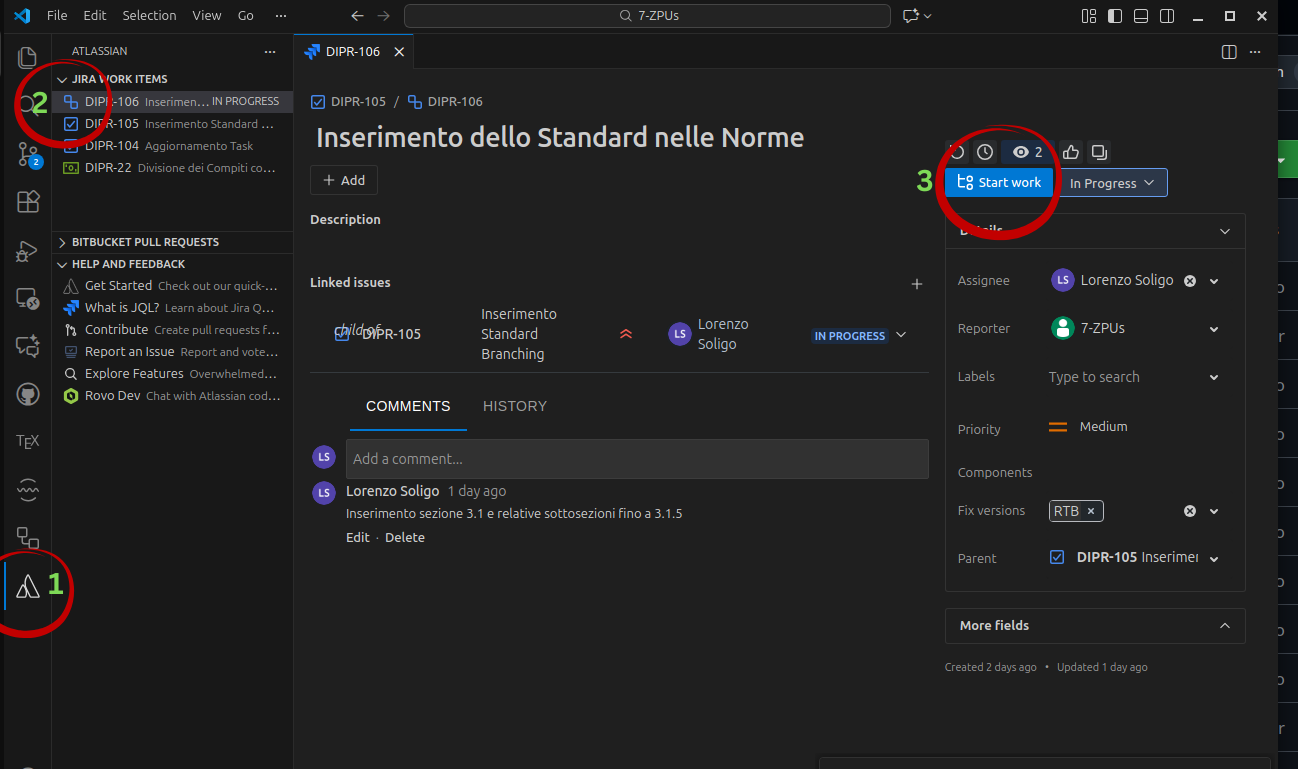
\includegraphics[width=1\textwidth]{../../assets/estensioneJira.png}
              \caption{Creazione del branch di lavoro tramite estensione Jira in VSCode}
          \end{figure}
    \item Quando è necessario \textbf{effettuare un commit} è obbligatorio utilizzare lo
          Smart Commit. Più in \ref{Jira}.
    \item Una volta completata la task, è necessario \textbf{creare la PR} verso la
          branch \textit{"in\_lavorazione"} di riferimento mettendo come revisore il
          membro del gruppo designato.\\ Per esempio, una volta completata la stesura di
          un verbale viene creata una PR verso \textit{verbali\_in\_lavorazione} e se
          questa viene approvata, il documento sarà pronto per la revisione finale del
          responsabile che si occuperà del merge con il \textit{main} in sede di
          milestone.\\
          \begin{figure}[H]
              \label{PR1}
              \centering
              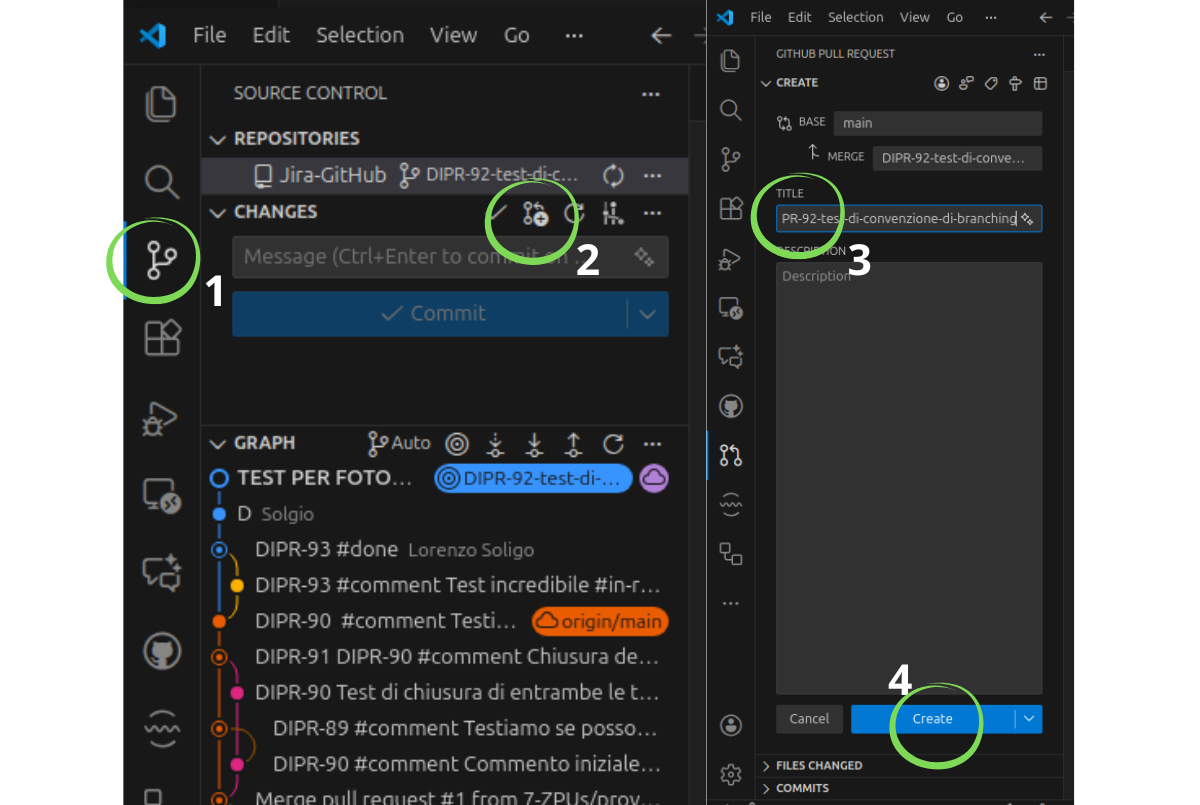
\includegraphics[width=1.1\textwidth]{../../assets/PRDocs1.png}
              \caption{Creazione della PR verso l'issue branch \textit{in\_lavorazione}}
          \end{figure}
\end{enumerate}

\paragraph{Procedura: Controllo della configurazione} \label{procedureControlloConfig}
Una volta effettuata una modifica nel branch relativo alla task, l'autore crea una Pull Request (PR) dal
branch associato alla task verso il branch di riferimento
\textit{x\_in\_lavorazione} (dove x è il nome del CI), impostando come revisore
il membro del gruppo designato alla verifica di tale task. Il revisore ha il
compito di controllare che la modifica sia corretta e conforme alle norme
definite, e di approvare o rifiutare la PR in base alla sua valutazione. \\ A
questo punto si verificano i seguenti scenari:
\begin{itemize}
    \item \textbf{Approvazione}: Il revisore procede con l'approvazione delle modifiche e la chiusura della PR tramite l'opzione "Create Merge Commit". Inoltre, specifica nello smart commit la direttiva "\#done" per chiudere automaticamente la relativa task su Jira.
          \begin{figure}[H]
              \label{PR2}
              \centering
              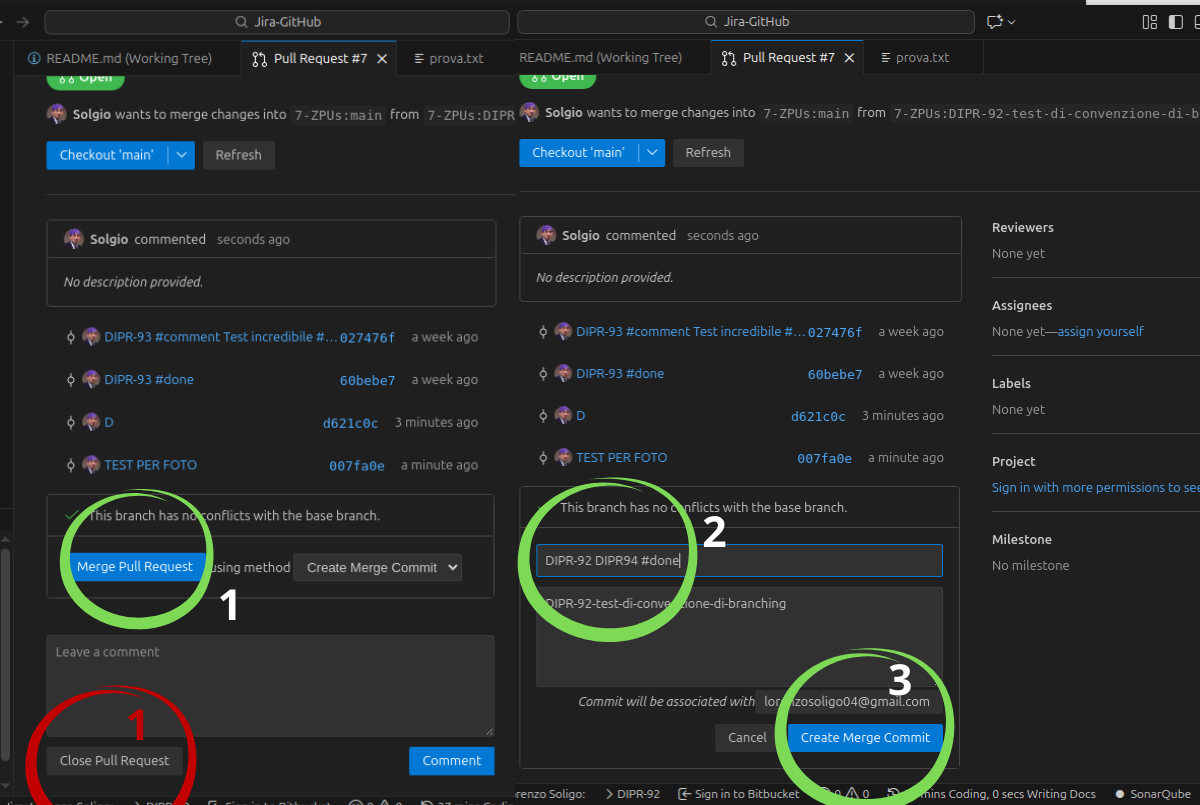
\includegraphics[width=1\textwidth]{../../assets/PRDocs2.png}
              \caption{Chiusura della PR tramite "Create Merge Commit"}
          \end{figure}
    \item \textbf{Richiesta di modifiche}: Il revisore fornisce un feedback puntuale all'autore tramite la funzione di review di GitHub. Una volta inseriti i commenti necessari all'autore, il revisore completa la review con l'esito: \textit{"Request changes"}. L'autore provvede a correggere i punti segnalati o a discuterne eventualmente tramite l'apposita sezione. Il revisore provvede ad una nuova revisione dei cambiamenti. Questo ciclo si ripete fino a quando i cambiamenti non vengono approvati.
    \item \textbf{Rifiuto}: Se la task viene annullata il revisore completa la review con l'esito: \textit{"Close with comment"}, inserendo un commento che spiega le motivazioni del rifiuto.
\end{itemize}

\paragraph{Smart Commit} \label{smartcommit}
La necessità di tracciamento delle attività richiede l'adozione capillare degli
Smart Commit per collegare i commit GitHub alle issue Jira. Questo permette di
aggiornare automaticamente lo stato delle task e rendicontare il tempo.

La sintassi obbligatoria è:
\begin{verbatim}
DIPR-<numero issue> #time <nd nh nm> #<stato> #comment <Descrizione> 
\end{verbatim}

\textbf{Regole di applicazione:}
\begin{enumerate}
    \item \textbf{Time Tracking:} L'inserimento del tempo (\texttt{\#time}) deve seguire il formato \textit{nd nh nm} (giorni, ore, minuti).
    \item \textbf{Transizioni di Stato:} Utilizzare i tag \texttt{\#start-progress}, \texttt{\#start-review}, \texttt{\#complete} per avanzare il \glossario{workflow} su Jira.
    \item \textbf{Pull Request:} Nelle PR è vietato inserire il tag \texttt{\#time} per evitare la doppia contabilizzazione delle ore lavorative.
    \item \textbf{Issue Multiple:} È possibile agire su più issue in un singolo commit separandole con spazi (utile per chiudere issue di sviluppo e verifica contemporaneamente).
\end{enumerate}

\paragraph{Standard per le Branch} \label{stdBranch}
Per garantire una gestione ordinata e coerente del codice e della
documentazione, il Team adotta il seguente standard per la denominazione dei
branch in GitHub:
\begin{itemize}
    \item La creazione del branch deve avvenire preferibilmente in modo automatico
          tramite l'integrazione Jira-VSCode (vedi §\ref{conf_vscode}).
    \item Il formato obbligatorio è:
          \begin{verbatim}
    DIPR-<numero issue>-<descrizione-breve>
    \end{verbatim}
    \item È necessario scegliere una descrizione breve che identifichi chiaramente il contenuto della modifica.
\end{itemize}

\paragraph{Strumenti}
\begin{itemize}
    \item \textbf{Git/GitHub:} per la gestione di PR e branch.
    \item \textbf{Jira:} per definire e tracciare i CIs e le relative task di modifica.
\end{itemize}

\subsubsection{Attività: Registrazione delle Configurazioni} \label{versionamento_identificazione}
Questa attività definisce le regole per la registrazione dei cambiamenti e il
versionamento dei CIs.

\textit{Nota}: il concetto di versione di un documento non corrisponde a quello di versione su GitHub.
Per versione in questa sezione si intende una versione stabilita come conseguenza di modifiche apportate all'artefatto di riferimento. Concetto che non coincide con quello di versione all'interno di GitHub.

\paragraph{Procedura: Registrazione delle Modifiche}\label{versione}
Per ogni modifica apportata a uno CI, è necessario documentare le seguenti
informazioni, all'interno della sezione denominata "Tabella di Versionamento",
situata all'inizio di ogni documento.\\Al suo interno vi sono:
\begin{itemize}
    \item Numero di versione
    \item Data della modifica (di più in \ref{convenzioniNomiDate})
    \item Autore della modifica
    \item Verificatore della modifica
    \item Descrizione della modifica, con riferimento preciso, al paragrafo o sezione
          interessata.
\end{itemize}
Per la numerazione delle versioni si adotta lo standard che segue:
\begin{itemize}
    \item \textbf{MAJOR} viene incrementato per modifiche sostanziali che introducono cambiamenti significativi o incompatibili con le versioni precedenti.
    \item \textbf{MINOR} viene incrementato per l'aggiunta di nuove funzionalità o miglioramenti che non compromettono la compatibilità con le versioni precedenti.
    \item \textbf{PATCH} viene incrementato per correzioni di bug, miglioramenti minori o modifiche che non influenzano le funzionalità principali del documento.
\end{itemize}

Ogni volta che viene apportata una modifica ad uno CI, è necessario aggiornare
la tabella di versionamento con le informazioni sopra descritte. Lo scatto di
versione avviene solamente in seguito all'approvazione delle modifiche da parte
del verificatore stabilito.

\paragraph{Strumenti}
\begin{itemize}
    \item \textbf{GitHub:} per tracciare le modifiche e collegarle alle issue Jira.
    \item \textbf{Jira:} per tracciare le task che portano alla modifica degli artefatti della baseline.
\end{itemize}

\subsubsection{Ruoli}
Vengono qui raccolti per praticità i ruoli coinvolti del processo di gestione
della configurazione, con una breve descrizione delle responsabilità di
ciascuno.

\begin{table}[H]
    \begin{adjustwidth}{-4cm}{-4cm}
        \centering
        \begin{spacing}{1.1}
            \begin{tabular}{|c|c|}
                \hline
                \textbf{Ruolo}           & \textbf{Specifica}                                                                                                                                                                                                    \\
                \hline
                Responsabile di progetto & \begin{tabular}[c]{@{}p{10cm}@{}}Figura coordinativa del gruppo che si occupa della identificazione, assegnazione e controllo di avanzamento dei task di modifica.\end{tabular}                                       \\
                \hline
                Amministratore           & \begin{tabular}[c]{@{}p{10cm}@{}}Si occupa del controllo dell'utilizzo corretto degli strumenti per la gestione delle configurazione. È il referente per l'uso corretto degli strumenti.\end{tabular}                 \\
                \hline
                Verificatore             & \begin{tabular}[c]{@{}p{10cm}@{}}Responsabile del controllo in seguito alle modifiche. È suo il compito di verificare che le modifiche apportate siano conformi alle norme e agli standard del progetto.\end{tabular} \\
                \hline
                Esecutore dell'attività  & \begin{tabular}[c]{@{}p{10cm}@{}}Esegue le attività di modifica seguendo le convenzioni definite come l'uso di Smart Commit e delle Pull Request.\end{tabular} \\
                \hline
            \end{tabular}
        \end{spacing}
    \end{adjustwidth}
\end{table}

\subsection{Processo di verifica}
Il processo di verifica è oggettivo e tecnico; ha lo scopo di accertare che i prodotti realizzati
(documenti e codice) siano conformi ai requisiti specificati e corretti nella loro implementazione.
La verifica viene svolta non solo su elementi software ma anche documentali.
A tal proposito, la parte di verifica riguardante gli artefatti software verrà affrontata successivamente al
raggiungimento della milestone RTB. E' importante sottolineare che il ruolo
della verifica differisce da quello della validazione. La verifica si concentra
sulla correttezza di quanto prodotto, mentre la validazione si focalizza
sull'adeguatezza del prodotto rispetto alle esigenze del cliente. La verifica è
un processo interno al team, mentre la validazione coinvolge anche la
committente.

\subsubsection{Analisi statica}
L'analisi statica consiste nell'esaminare codice e documentazione senza
eseguire il software, al fine di individuare errori o non conformità alle norme. L'analisi statica viene effettuata mediante:
\begin{itemize}
    \item \textbf{Walkthrough}: analisi esplorativa del codice o del testo senza conoscenza preventiva della posizione dell'errore. I verificatori individuano le anomalie, mentre la correzione è a carico degli autori.

    \item \textbf{Inspection}: analisi mirata di specifiche porzioni di codice o testo in cui si sospetta la presenza di errori, basata sull'esperienza e su conoscenze pregresse. Assai più efficiente ed automatizzabile rispetto al walkthrough, ma richiede esperienza, spesso a valle di più walkthrough.
\end{itemize}

\subsubsection{Analisi dinamica}
L'analisi dinamica consiste nell'eseguire il software per verificarne il
comportamento rispetto ai requisiti specificati. I test devono essere
ripetibili e automatizzabili, isolati e il più efficienti possibili per garantire
efficienza.

\subsubsection{Attività: Verifica documentale}
La verifica documentale consiste nel controllo dei documenti prodotti prima
della loro approvazione. La verifica avviene su più fronti:
\begin{itemize}
    \item \textbf{Contenuto}: correttezza dei contenuti, che devono soddisfare le aspettative definite per la task di riferimento
    \item \textbf{Correttezza grammaticale e leggibilità}: i documenti devono essere scritti in modo chiaro, con una grammatica corretta e un livello di leggibilità adeguato al pubblico di riferimento.
    \item \textbf{Aderenza alle linee guida}: i documenti devono rispettare le linee guida stabilite per la produzione della documentazione, come descritto in \ref{lineeGuidaProduzioneDocs}.
\end{itemize}

\paragraph{Procedura: Verifica del contenuto documentale}
La verifica del contenuto documentale avviene tramite \textbf{walkthrough}, con
eventuale ausilio di LLM. Il controllo del contenuto avviene
corrispondentemente alle aspettative definite per la singola task. E' buona
prassi assegnare come verificatore un membro che si ritiene più competente in
merito al contenuto del documento, in modo da garantire una verifica più
accurata e puntuale. Ogni documento deve rispettare quanto descritto in
\ref{lineeGuidaProduzioneDocs}.

\paragraph{Procedura: Verifica di correttezza grammaticale e di leggibilità}
La verifica di correttezza grammaticale e di leggibilità avviene tramite script
automatizzati. Lo script è contenuto nella directory \texttt{scripts}. Oltre al
controllo locale, una volta aperta la Pull Request per candidare le modifiche,
vengono eseguiti dei workflow automatizzati che prevedono un controllo di
grammatica e leggibilità tramite Aspell e Textstat.\\

\paragraph{Procedura: Verifica di aderenza alle linee guida}
La verifica di aderenza è attuata in forma di checklist. Il verificatore, durante la revisione del documento, si assicura che sia conforme a quanto specificato in \ref{lineeGuidaProduzioneDocs}

\paragraph{Strumenti}
\begin{itemize}
    \item \textbf{LLM} per il supporto alla verifica del contenuto, in particolare per l'analisi di coerenza, completezza e aderenza alle linee guida.
    \item \textbf{Aspell} per il controllo ortografico, utilizzato negli script automatizzati (Github Action).
    \item \textbf{Textstat} per il controllo di leggibilità, utilizzato negli script automatizzati (Github Action).
\end{itemize}

\subsubsection{Attività: Verifica del codice}
La verifica statica del codice avviene grazie all'utilizzo di SonarQube, che permette di individuare errori, vulnerabilità e code smell nel codice sorgente. 
Il processo di verifica del codice è integrato nel workflow di sviluppo, con l'esecuzione automatica dei controlli ad ogni push o pull request.\\
Inoltre, il Team inoltre può consultare la dashboard di SonarQube per monitorare la qualità del codice a livello di branch e di progetto.\\
La verifica dinamica del codice come già anticipato nella sezione \ref{test}, avviene in tre fasi, descritte a seguire.

\paragraph{Procedura: Test di unità}
Ogni componente software deve essere accompagnato da un test di unità che ne verifichi il comportamento in isolamento. Visto la natura del test, eventuali dipendenze vengono sostituite da \glossario{mock}.\\
Utilizzando i comandi Angular, nella sezione frontend, è possibile generare automaticamente i file di test da popolare. Si consiglia quindi di sfruttare al massimo le potenzialità di Angular.

\paragraph{Procedura: Test di integrazione}
I test di integrazione verificano l'interazione tra più componenti, assicurando che funzionino correttamente insieme. È utile effettuare test di integrazione graduale man mano che si sviluppano le componenti.\\
In questo caso, i mock vengono limitati a componenti al di sotto del livello di integrazione testato.

\paragraph{Procedura: Test end-to-end di sistema}
I test end-to-end verificano il sistema nella sua interezza, simulando l'interazione dell'utente con l'interfaccia grafica e verificando che tutte le componenti funzionino correttamente insieme.\\
Per facilitare l'esecuzione il testing, viene utilizzato il pattern Page Object, che permette di astrarre l'interazione con l'interfaccia grafica in classi dedicate, migliorando la manutenibilità dei test e riducendo la duplicazione di codice.
Così facendo, e utilizzando selettori stabili come \textit{data-testid}, non si dipende da elementi di interfaccia variabili come etichette o parametri grafici.
\subparagraph{POM pattern per i test E2E}
Il pattern Page Object Model (POM) è una metodologia di progettazione per i test end-to-end che prevede la creazione di classi dedicate per rappresentare le pagine dell'applicazione. 
Ogni classe contiene metodi che rappresentano le azioni che un utente può eseguire sulla pagina, come cliccare su un pulsante o inserire testo in un campo.\\
Il flusso di interazione utente viene quindi rappresentato attraverso l'invocazione di questi metodi, rendendo i test più leggibili e manutenibili.\\
Inoltre, il POM consente di centralizzare la gestione dei selettori, raggruppando in un'unica classe tutti i selettori.
\\ Per il tracciamento dei test di sistema è stato creato un piccolo script che, a  partire dai file di test e i codici di test, genera un file di con indicazioni sullo stato di copertura e indicazione delle coordinate test file di un determinato test.

\subsubsection{Ruoli}
Vengono qui raccolti per praticità i ruoli coinvolti del processo di verifica,
con una breve descrizione delle responsabilità di ciascuno.

\begin{table}[H]
    \begin{adjustwidth}{-4cm}{-4cm}
        \centering
        \begin{spacing}{1.1}
            \begin{tabular}{|c|c|}
                \hline
                \textbf{Ruolo}           & \textbf{Specifica}                                                                                                                                                                               \\
                \hline
                Responsabile di progetto & \begin{tabular}[c]{@{}p{10cm}@{}}Stabilisce, pianifica, coordina e monitora le attività di verifica del prodotto.\end{tabular}                                                                   \\
                \hline
                Verificatore             & \begin{tabular}[c]{@{}p{10cm}@{}}Garante della qualità dei prodotti, verifica i contenuti, la forma e la struttura dei documenti secondo le norme comuni e specifiche del progetto.\end{tabular} \\
                \hline
            \end{tabular}
        \end{spacing}
    \end{adjustwidth}
\end{table}

\subsection{Processo di validazione}
La validazione è un processo soggettivo e orientato all'utente, con cui si verifica che il prodotto sviluppato
soddisfi i requisiti e le aspettative della proponente. La validazione si
focalizza sull'adeguatezza del prodotto rispetto alle esigenze del cliente. Serve a capire
se il software soddisfa effettivamente i requisiti lato utente.

\subsubsection{Attività: Pianificazione della validazione}
Questa attività prevede la definizione delle strategie e dei criteri di
validazione, nonché la pianificazione delle attività correlate. La
pianificazione della validazione avviene contestualmente alla pianificazione
dello sviluppo, in modo da garantire che le attività di validazione siano
integrate nel ciclo di sviluppo.

\paragraph{Procedura: Pianificazione della validazione}
Per pianificare efficacemente la validazione, il Team segue i seguenti
passaggi:
\begin{enumerate}
    \item Identificazione dei requisiti utente chiave da validare, in collaborazione con la
          proponente, per garantire che le aspettative del cliente siano chiaramente
          comprese e integrate nella pianificazione.
    \item Definizione dei criteri di accettazione, specificando i
          risultati attesi e le condizioni di successo per la validazione attraverso i test di accettazione.
    \item Assegnazione delle responsabilità per le attività di validazione, identificando
          i membri del team che si occuperanno della progettazione e dell'esecuzione dei
          test di validazione.
\end{enumerate}

\paragraph{Strumenti}
\begin{itemize}
    \item \textbf{Jira:} per la gestione delle attività di validazione, con la creazione di task specifici per la pianificazione e l'esecuzione dei test.
    \item \textbf{\LaTeX:} per la definizione dei test di accettazione nel documento Piano di Qualifica.
    \item \textbf{Vitest:} per la definizione e esecuzione dei test di unità e di integrazione
    \item \textbf{Playwright:} per la definizione e esecuzione dei test end-to-end di sistema.
    \item \textbf{SonarQube:} per la verifica statica del codice, integrata nel processo di sviluppo.
\end{itemize}

\subsubsection{Attività: Definizione dei test di accettazione}
In questa attività vengono progettati i casi di test finalizzati a verificare
che il sistema soddisfi le esigenze della proponente.

\paragraph{Procedura: Definizione dei test di accettazione}
Per definire i test di accettazione, il Team segue i seguenti passaggi:
\begin{enumerate}
    \item Raccolta dei requisiti (utente) chiave identificati durante la fase di analisi per
          comprendere le funzionalità e i comportamenti attesi del sistema.
    \item Progettazione dei casi di test di accettazione, specificando le condizioni di
          test, i dati di input, i risultati attesi e i criteri di successo per ogni
          caso.
    \item Revisione dei casi di test con la proponente per garantire che siano allineati
          con le aspettative del cliente e che coprano adeguatamente i requisiti chiave.
\end{enumerate}

\paragraph{Strumenti}
\begin{itemize}
    \item \textbf{Jira:} per la creazione e la gestione delle attività di test di accettazione, con la possibilità di tracciare l'esecuzione e i risultati dei test.
    \item \textbf{Analisi dei Requisiti:} come riferimento per i requisiti da validare.
\end{itemize}

\subsubsection{Attività: Esecuzione dei test di accettazione}
Questa attività prevede l'esecuzione dei test di accettazione pianificati, la
raccolta dei risultati e l'analisi degli esiti per determinare se il prodotto
soddisfa i requisiti stabiliti.

\paragraph{Procedura: Esecuzione dei test di accettazione}
Per eseguire i test di accettazione, il Team segue i seguenti passaggi:
\begin{enumerate}
    \item Preparazione dell'ambiente di test, assicurandosi che sia configurato
          correttamente e che tutti i componenti necessari siano disponibili per
          l'esecuzione dei test.
    \item Esecuzione dei casi di test di accettazione, seguendo le condizioni e i dati di
          input specificati, e registrando i risultati ottenuti.
    \item Analisi dei risultati dei test, confrontando i risultati ottenuti con quelli
          attesi per determinare se il prodotto soddisfa i requisiti (utente) e identificare
          eventuali problemi o aree di miglioramento.
\end{enumerate}

\paragraph{Strumenti}
\begin{itemize}
    \item \textbf{Jira:} Per tracciare l'avanzamento delle attività di validazione.
    \item \textbf{Piano di Qualifica:} Per la registrazione degli esiti dei test.
\end{itemize}

\subsubsection{Ruoli}
Vengono qui raccolti per praticità i ruoli coinvolti del processo di
validazione, con una breve descrizione delle responsabilità di ciascuno.

\begin{table}[H]
    \begin{adjustwidth}{-4cm}{-4cm}
        \centering
        \begin{spacing}{1.1}
            \begin{tabular}{|c|c|}
                \hline
                \textbf{Ruolo}           & \textbf{Specifica}                                                                                                                                                                                                                                                                                       \\
                \hline
                Responsabile di progetto & \begin{tabular}[c]{@{}p{10cm}@{}}Stabilisce, pianifica, coordina e monitora le attività di validazione del prodotto. È inoltre il membro del gruppo che ha il compito di monitorare il corretto svolgimento delle attività in riferimento ai requisiti e ai test di accettazione stabiliti.\end{tabular} \\
                \hline
                Amministratore           & \begin{tabular}[c]{@{}p{10cm}@{}}Controlla che il sistema di test sia configurato in modo corretto. L'obiettivo è rendere la validazione più affidabile, ripetibile e automatizzabile.\end{tabular}                                                                                                      \\
                \hline
            \end{tabular}
        \end{spacing}
    \end{adjustwidth}
\end{table}

\subsection{Processo di revisione congiunta}\label{proc_revisione_congiunta}
Il processo di revisione congiunta è un'attività sincrona tra i membri del
gruppo, finalizzata al terminare un'insieme di sviluppo o di documentazione
coese tra loro. Questa attività risulta particolarmente utile se eseguita in
concomitanza del raggiungimento di una milestone. Verosimilmente, oggetti della
revisione congiunta coincideranno con dei Configuration Items. Il processo di
revisione congiunta prevede la partecipazione di un sottoinsieme dei membri del
gruppo, selezionati in base al loro coinvolgimento nelle attività che hanno
contribuito alle modifiche del suddetto Configuration Item.

\subsubsection{Attività: Pianificazione}
La pianificazione della revisione congiunta è stabilita dal responsabile in
collaborazione con i membri del team che si sono occupati dello sviluppo del
Configuration Item. L'attività viene pianificata secondo quanto scritto in
§\ref{gestione_processi_organizzativi}.

\paragraph{Procedura: Identificazione dei partecipanti}
Il responsabile identifica i membri del team che parteciperanno alla revisione
congiunta, tenendo conto dei seguenti criteri:
\begin{enumerate}
    \item \textbf{Coinvolgimento diretto}: priorità ai membri che hanno contribuito direttamente allo sviluppo del Configuration Item.
    \item \textbf{Competenza tecnica}: includere membri con conoscenze specifiche dell'area di revisione (architetturale, documentale, etc.).
\end{enumerate}
Una volta identificati, i partecipanti vengono formalmente comunicati tramite i canali asincroni.

\paragraph{Procedura: Identificazione del materiale oggetto di revisione}
Il responsabile, in collaborazione con il team, identifica e documenta il
materiale da sottoporre a revisione congiunta:
\begin{enumerate}
    \item \textbf{Determinazione del Configuration Item}: viene identificato il CI (documento, componente software, set di test, etc.) che ha raggiunto una milestone o uno stato di maturità sufficiente per la revisione congiunta.
    \item \textbf{Comunicazione degli obiettivi di revisione}: vengono stabiliti chiaramente gli obiettivi della revisione.
\end{enumerate}

\paragraph{Procedura: Pianificazione della sessione di revisione}
Il responsabile pianifica la sessione di revisione congiunta seguendo i
seguenti passaggi:
\begin{enumerate}
    \item \textbf{Definizione della data e dell'ora}: viene stabilita una data e un'ora che sia compatibile con la disponibilità di tutti i partecipanti identificati. Si preferisce una sessione sincrona in modo da favorire discussioni approfondite e chiarimenti immediati.
    \item \textbf{Durata stimata}: viene stimata la durata della sessione in base alla complessità del CI e al numero di partecipanti, con una media di 1-2 ore.
    \item \textbf{Modalità di conduzione}: viene stabilito il formato della revisione:
          \begin{itemize}
              \item \textbf{In presenza}: se possibile, per favorire una comunicazione più naturale e una collaborazione più stretta.
              \item \textbf{Remota tramite Discord}: utilizzando il server Discord del gruppo con canale dedicato per la sessione.
              \item \textbf{Ibrida}: combinazione di partecipanti in presenza e remoti, utilizzando Discord e uno schermo condiviso.
          \end{itemize}
\end{enumerate}

\paragraph{Strumenti}
\begin{itemize}
    \item \textbf{Jira}: Per la creazione di task dedicate alle revisioni congiunte e il tracciamento delle attività correlate.
    \item \textbf{Discord}: Per la comunicazione dei dettagli della revisione e la condivisione di aggiornamenti in tempo reale.
    \item \textbf{GitHub}: Per l'accesso al materiale di revisione (documenti, codice, branch).
\end{itemize}

\subsubsection{Attività: Esecuzione della revisione congiunta}
\paragraph{Procedure: Definizione dell'ordine di revisione del materiale}
La fase iniziale della revisione prevede una piccola pianificazione dell'ordine
di revisione del materiale, che tenga conto della complessità e delle relazioni
tra le varie parti che lo compongono. Si lascia la libertà a chi conduce la
revisione di stabilire l'ordine e la logica più adatta al caso specifico,
tenendo conto dei seguenti criteri:
\begin{enumerate}
    \item \textbf{Logica di sviluppo}: seguire l'ordine in cui le parti sono state sviluppate o documentate, per facilitare la comprensione del processo di sviluppo e delle scelte progettuali.
    \item \textbf{Relazioni tra le parti}: iniziare con le parti più generali o di alto livello (ad esempio, l'architettura generale) per poi passare a quelle più specifiche (ad esempio, dettagli di implementazione o sezioni di documentazione).
    \item \textbf{Punti critici}: dare priorità alla revisione di parti che sono state identificate come potenzialmente problematiche o che hanno subito modifiche significative, per garantire che eventuali problemi vengano individuati e risolti tempestivamente.
\end{enumerate}

\paragraph{Procedura: Revisione del materiale}
Durante la revisione ai partecipanti esaminano attentamente il materiale,
discutendo eventuali dubbi, criticità o proposte di miglioramento. Ogni
problema emerso durante la revisione viene comunicato al responsabile, che si
occupa poi di pianificare le attività di risoluzione assieme ai revisori.

\paragraph{Strumenti}
\begin{itemize}
    \item \textbf{Discord}: Per la comunicazione durante la sessione di revisione, con canale dedicato e possibilità di condividere schermi e documenti in tempo reale.
    \item \textbf{GitHub}: Per l'accesso al materiale di revisione.
    \item \textbf{LiveShare}: Per la condivisione degli ambienti di lavoro e l'editing collaborativo in tempo reale.
\end{itemize}

\subsubsection{Ruoli}
Vengono qui raccolti per praticità i ruoli coinvolti del processo di revisione
congiunta, con una breve descrizione delle responsabilità di ciascuno.

\begin{table}[H]
    \begin{adjustwidth}{-4cm}{-4cm}
        \centering
        \begin{spacing}{1.1}
            \begin{tabular}{|p{5cm}|p{10cm}|}
                \hline
                \textbf{Ruolo}                                      & \textbf{Specifica}                                                                                                                                                                                                                  \\
                \hline
                Responsabile di progetto                            & \begin{tabular}[c]{@{}p{10cm}@{}}Coordinatore dell'attività di revisione congiunta\end{tabular} \\
                \hline
                Tutti i membri del gruppo coinvolti nella revisione & \begin{tabular}[c]{@{}p{10cm}@{}}Partecipano attivamente alla revisione congiunta, esaminando i materiali e contribuendo alle discussioni\end{tabular}                                                                             \\
                \hline
                Amministratore & \begin{tabular}[c]{@{}p{10cm}@{}}Garantisce l'accesso al materiale soggetto a revisione\end{tabular} \\
                \hline
            \end{tabular}
        \end{spacing}
    \end{adjustwidth}
\end{table}

\subsection{Processo di garanzia della qualità}\label{gestione_qualita}
Il processo di garanzia della qualità sovrintende all'applicazione sistematica
delle metriche definite e all'integrazione tra i processi di garanzia della
qualità, verifica, validazione e miglioramento per garantire la qualità
complessiva del prodotto finale e dei processi. \\Questo processo coordina
tutte le attività volte a mantenere e migliorare gli standard qualitativi
durante l'intero ciclo di vita del progetto.

\subsubsection{Attività: Pianificazione della qualità}\label{pianificazione_qualita}

\paragraph{Procedura: Definizione di metriche e soglie}
Il responsabile coordina la pianificazione degli obiettivi di qualità:
\begin{enumerate}
    \item \textbf{Definizione delle metriche di processo}: vengono stabilite le metriche chiave da monitorare per ciascun processo implementato. La scelta deve tenere conto di: grado di automazione, facilità di raccolta, valore aggiunto nella sua misurazione. La misurazione di una metrica comporta sempre, benché talvolta minimo, un costo. Per questo motivo va fatta una selezione attenta e accurata. Per la definizione è bene attenersi a metriche riconosciute e consolidate, prevenendo l'introduzione di errori di definizione o di interpretazione.
    \item \textbf{Definizione delle metriche di prodotto}: vengono stabilite le metriche chiave da monitorare per il prodotto software finale. La selezione avviene con gli stessi criteri delle metriche di processo; in aggiunta si sottolinea come la metrica debba essere pertinente al dominio applicativo.
    \item \textbf{Definizione delle soglie di accettabilità}: per ogni metrica definita, vengono stabilite le soglie di accettabilità che indicano i livelli minimi di qualità da raggiungere. Le soglie devono essere realistiche e basate su dati storici o benchmark di settore, per garantire che siano sfidanti ma raggiungibili.
    \item \textbf{Definizione dei valori di ottimalità}: per ogni metrica, vengono stabiliti i valori di ottimalità che rappresentano i livelli di qualità ideali da raggiungere. Questi valori servono come riferimento per il miglioramento continuo e per motivare il team a superare gli standard minimi.
\end{enumerate}

Gli obiettivi di qualità vengono documentati e comunicati a tutto il team nel documento Piano di Qualifica.
La definizione delle metriche è presente rispettivamente:
\begin{itemize}
    \item Per le metriche di processo, nella sezione \ref{qualita_processo}.
    \item Per le metriche di prodotto, nella sezione \ref{qualita_prodotto}.
\end{itemize}

\subsubsection{Attività: Monitoraggio continuo}\label{monitoraggio_continuo}

\paragraph{Procedura: Monitoraggio}
Durante lo svolgimento dei periodi, la qualità viene monitorata costantemente
attraverso:
\begin{enumerate}
    \item \textbf{Controllo automatizzato:}
          \begin{itemize}
              \item Le GitHub Actions eseguono verifiche automatiche ad ogni commit (indice
                    Gulpease, build success rate, etc.)
          \end{itemize}
    \item \textbf{Controllo manuale:}
          \begin{itemize}
              \item I verificatori eseguono revisioni del codice e della documentazione secondo le
                    procedure definite
              \item Vengono eseguiti test manuali per verificare usabilità e funzionalità
              \item Si monitora l'aderenza alle soglie stabilite
          \end{itemize}
    \item \textbf{Utilizzo del Cruscotto di Qualità:}
          \begin{itemize}
              \item Le metriche raccolte vengono visualizzate su un cruscotto dedicato all'interno
                    del Piano di Qualifica
                    % \item La Dashboard Jira personalizzata (\ref{knowladge_base}) fornisce una vista in tempo reale dello stato delle metriche
              \item Vengono monitorati trend e deviazioni rispetto agli obiettivi
          \end{itemize}
\end{enumerate}

\subsubsection{Attività: Valutazione periodica}\label{valutazione_periodica}
La valutazione periodica al fine del miglioramento continuo. Esistono però
diverse forme di valutazione periodica.
\paragraph{Procedura: Review settimanale}
Durante le riunioni di team, vengono discusse brevemente le metriche principali
e le eventuali criticità emerse. Questa review è scaturita dalla analisi del
cruscotto e delle sue metriche.
\paragraph{Procedura: Review di fine Sprint:}
Al termine di ogni Sprint:
\begin{itemize}
    \item Si confrontano le metriche ottenute con gli obiettivi pianificati
    \item Si analizzano le cause di eventuali scostamenti significativi
    \item Si valuta l'efficacia delle azioni correttive implementate
    \item Si aggiorna il cruscotto di qualità nel Piano di Qualifica
\end{itemize}
\paragraph{Procedura: Review di milestone}
In preparazione delle milestone:
\begin{itemize}
    \item Si effettua una valutazione complessiva della qualità raggiunta
    \item Si verifica il rispetto di tutti i requisiti di qualità obbligatori
          % \item Si producono report dettagliati per committente e proponente
\end{itemize}

\subsubsection{Attività: Azioni correttive}\label{azioni_correttive}

\paragraph{Procedura: Identificazione della deviazione e analisi delle cause}
Attraverso il monitoraggio continuo o le review periodiche è possibile
identificare eventuali deviazioni dagli standard di qualità imposti.
\paragraph{Procedura: Pianificazione dell'intervento}
La pianificazione del piano di intervento correttivo si differenzia in in base
al grado di importanza, complessità ed estensione delle deviazioni.
\begin{itemize}
    \item Per deviazioni minori: si assegna una issue correttiva al membro responsabile
    \item Per deviazioni significative: il responsabile convoca una sessione dedicata per
          pianificare l'intervento
\end{itemize}
\paragraph{Procedura: Implementazione e verifica}
L'azione correttiva viene implementata in modo specifico alla deviazione

\paragraph{Linee guida di gestione della qualità}
Le seguenti linee guida orientano il Team nella gestione sistematica della
qualità:
\begin{enumerate}
    \item \textbf{Prevenzione > Correzione:} Si privilegia l'adozione di pratiche preventive (code review, test automatici, standard di codifica) rispetto alla correzione a posteriori
    \item \textbf{Automazione quando possibile:} Le verifiche ripetitive vengono automatizzate per ridurre errori umani e liberare tempo per attività a maggior valore aggiunto
    \item \textbf{Tracciabilità completa:} Ogni decisione relativa alla qualità, ogni deviazione e ogni azione correttiva vengono documentate per garantire tracciabilità
    \item \textbf{Miglioramento continuo:} Le metriche e le procedure di qualità vengono periodicamente riviste e aggiornate in base all'esperienza accumulata
    \item \textbf{Responsabilità condivisa:} La qualità è responsabilità di tutti i membri del team, non solo dei verificatori
\end{enumerate}

\subsubsection{Metriche di gestione della qualità}\label{metriche_gestione_qualita}
L'efficacia del processo di gestione della qualità viene valutata attraverso la
\textbf{percentuale di metriche rispettate}. Questa indica il numero di
metriche che soddisfano le soglie minime rispetto al totale delle metriche
monitorate

Questa meta-metrica viene rendicontata nel Piano di Qualifica insieme alle
metriche di processo e prodotto definite nella sezione \ref{metriche_qualita}.

\subsubsection{Strumenti}\label{strumenti_gestione_qualita}
\begin{itemize}
    \item \textbf{Piano di Qualifica}: Documento di riferimento per obiettivi, metriche e soglie di qualità
    \item \textbf{Jira} Per il monitoraggio in tempo reale dello stato delle metriche,
          il tracciamento delle non conformità, le azioni correttive e la condivisione di report di qualità con la proponente
    \item \textbf{GitHub Actions}: Per l'automazione delle verifiche di qualità (Gulpease, build, test)
    \item \textbf{Strumenti di analisi statica}: Per il calcolo automatico di metriche di codice (complessità, coverage, accoppiamento)
\end{itemize}

\subsubsection{Ruoli}
Vengono qui raccolti per praticità i ruoli coinvolti del processo di gestione
della qualità, con una breve descrizione delle responsabilità di ciascuno.
\begin{table}[H]
    \begin{adjustwidth}{-4cm}{-4cm}
        \centering
        \begin{spacing}{1.1}
            \begin{tabular}{|c|c|}
                \hline
                \textbf{Ruolo} & \textbf{Specifica}                                                                                                                                                       \\
                \hline
                Responsabile   & \begin{tabular}[c]{@{}c@{}} Coordina le attività di gestione della qualità e garantisce \\ il rispetto degli obiettivi definiti nel Piano di Qualifica, \\ verificando periodicamente le metriche riportate a cruscotto \end{tabular}     \\
                \hline
                Verificatori   & \begin{tabular}[c]{@{}c@{}} Eseguono le verifiche secondo le procedure definite e misurano \\ (se necessario manualmente) le metriche di \\ qualità di processo e prodotto \end{tabular}              \\
                \hline
                Amministratore & \begin{tabular}[c]{@{}c@{}} Configura e mantiene gli strumenti di automazione per il monitoraggio\\ della qualità (GitHub Actions, Jira) \end{tabular} \\
                \hline
                Tutti i membri & \begin{tabular}[c]{@{}c@{}} Contribuiscono al mantenimento della qualità seguendo \\ le norme e segnalando deviazioni dagli standard \end{tabular}                       \\
                \hline
            \end{tabular}
        \end{spacing}
    \end{adjustwidth}
\end{table}

\section{Processi Organizzativi}
\subsection{Processo di Gestione} \label{gestione_processi_organizzativi}
La gestione descrive le modalità di comunicazione interne ed esterne, i vari
ruoli e i loro compiti.

\subsubsection{Attività: Pianificazione}
L'attività di pianificazione riguarda per lo più il responsabile, il quale deve
adoperarsi per popolare il backlog con attività dettagliate e assegnabili alla
singola persona.
\paragraph{Procedura: Identificazione}\label{identificazioneTaskGestione}
E' necessario prima di ogni cosa capire quali sono le task da svolgere, le
dipendenze tra esse, le stime di tempo e risorse umane. L'identificazione
avviene durante le riunioni interne di gruppo di progetto, le quali sono
documentate in verbali. Ogni decisione presa viene riportata in una tabella
dedicata con un riferimento ad una Jira Issue. Vista l'impossibilità e la poca
utilità in certi casi di pianificare nel dettaglio ogni singola attività, vengono stabilite in
linea generale le macro attività da svolgere. Successivamente il responsabile
provvederà a scomporre in task atomiche queste ultime, comunicando
all'amministratore tutte le informazioni necessarie per inserirle in Jira. Le
informazioni sono:
\begin{itemize}
    \item Titolo della task
    \item Assegnatario
    \item Ruolo
    \item Priorità
    \item Data di scadenza
    \item Stima in ore
    \item Data di inizio
    \item Versione di correzione (RTB o PB)
    \item Relazioni di dipendenza con altre task
\end{itemize}

Successivamente l'amministratore provvederà a riportare quanto deciso dal
responsabile sulla piattaforma Jira.

\paragraph{Strumenti}
\begin{itemize}
    \item \textbf{Jira:} Per la gestione del backlog, la creazione e l'assegnazione delle task, e il monitoraggio dello stato di avanzamento.
    \item \textbf{GitHub:} Per la condivisione dei verbali di riunione e dei documenti di pianificazione.
    \item \textbf{Discord:} Per le discussioni interne durante la fase di pianificazione e per il coordinamento del team.
\end{itemize}

\subsubsection{Attività: Esecuzione e Controllo}
L'attività di esecuzione e controllo riguarda tutti i membri del team. Ognuno a
questo punto ha compiti chiari e ben definiti da svolgere entro determinate
scadenze.
\paragraph{Procedura: Controllo di Processo}
Il responsabile durante il periodo di esecuzione si occupa di monitorare lo
stato di avanzamento delle task in maniera periodica. Individua eventuali
rallentamenti, dipendenze non esaminate o problemi dei componenti del team, e
si adopera per risolverli. L'amministratore garantisce al responsabile la
continua misura degli indici di qualità di processo definiti in
\ref{metriche_qualita}.
\paragraph{Strumenti}
\begin{itemize}
    \item \textbf{Jira:} Per il monitoraggio dello stato di avanzamento delle task, l'identificazione di eventuali blocchi o ritardi, e la gestione delle dipendenze tra le attività.
    \item \textbf{Discord:} Per la comunicazione rapida e il coordinamento del team durante l'esecuzione delle attività, soprattutto in caso di problemi o necessità di riallineamento.
    \item \textbf{Cruscotto di controllo:} per la visualizzazione degli indici di qualità stabiliti.
\end{itemize}

\subsubsection{Attività: Retrospettiva}
L'attività di retrospettiva riguarda tutti i membri del team e si svolge
durante le riunioni interne di gruppo di progetto.
\paragraph{Procedura: Retrospettiva di periodo}
Ad ogni termine di Sprint, il team dedica una porzione della riunione alla
retrospettiva. Vengono analizzati i seguenti punti:
\begin{itemize}
    \item Cosa è andato bene durante lo Sprint: sia a livello organizzativo che
          esecutivo.
    \item Cosa è andato male: eventuali problemi riscontrati, difficoltà incontrate,
          e aree di miglioramento.
    \item Valutazione degli indici di qualità misurati durante lo Sprint
    \item Eventuale definizione di azioni correttive o migliorative.
\end{itemize}
Le decisioni prese durante la retrospettiva vengono documentate nell'apposita sezione dei verbali come definito in \ref{produzioneDocs}. È importante
che ogni membro del team partecipi attivamente alla retrospettiva, non limitandosi ad un atteggiamento passivo.

\paragraph{Strumenti}
\begin{itemize}
    \item \textbf{Cruscotto di controllo:} Per la condivisione dei verbali di retrospettiva e dei materiali di analisi.
    \item \textbf{Discord:} Per la discussione interna durante la retrospettiva e per il coordinamento del team.
    \item \textbf{Jira:} Per la creazione di eventuali task correttive o migliorative emerse durante la retrospettiva.
\end{itemize}

\subsubsection{Ruoli}
Vengono qui raccolti per praticità i ruoli coinvolti del processo di gestione, con una breve descrizione delle responsabilità di ciascuno.
\begin{table}[H]
    \begin{adjustwidth}{-4cm}{-4cm}
        \centering
        \begin{spacing}{1.1}
            \begin{tabular}{|c|c|}
                \hline
                \textbf{Ruolo} & \textbf{Specifica}                                                                           \\
                \hline
                Responsabile   & \begin{tabular}[c]{@{}c@{}} Gestisce la distribuzione di attività tra i membri,\\ assegnando le
                                     attività basandosi sull'ammontare \\ore rimasto per ogni ruolo ed ogni membro.\\ Si
                                     occupa inoltre della redazione dei verbali, della comunicazione\\ con la
                                     proponente e dell'aggiornamento del piano di progetto. \\È suo compito il controllo del cruscotto di controllo.\end{tabular} \\
                \hline
                Amministratore & \begin{tabular}[c]{@{}c@{}} Si occupa del corretto svolgimento del progetto, \\manutenendo
                                     l'infrastruttura, e controllando il corretto \\aderimento alle pratiche Sprint.\\
                                     Si occupa anche della scrittura delle norme di progetto \\e della creazione delle task su Jira.
                                    \\È suo compito anche il monitoraggio del funzionamento del cruscotto e\\ del recupero automatico delle metriche\end{tabular}      \\
                \hline
                Tutti i membri & \begin{tabular}[c]{@{}c@{}} Sono coinvolti nella retrospettiva di ogni Sprint.\end{tabular}      \\

                \hline
            \end{tabular}
        \end{spacing}
    \end{adjustwidth}
\end{table}

\subsection{Processo di Infrastruttura}
Il processo di Infrastruttura fornisce e mantiene il supporto tecnico, hardware e software, necessario per lo sviluppo e la gestione del progetto.

\subsubsection{Attività: Implementazione}\label{ImplementazioneInfrastruttura}
Per garantire un ambiente di lavoro efficiente, il Team definisce e documenta l'infrastruttura valutando ogni strumento e tecnologia in base ai seguenti vincoli normativi:
\begin{itemize}
    \item \textbf{Funzionalità e Prestazioni:} Lo strumento deve coprire esattamente le necessità del task senza appesantire il flusso di lavoro.
    \item \textbf{Costi e Vincoli di Tempo:} Viene data priorità a soluzioni gratuite, open-source o già fornite in licenza dall'Ateneo, con una curva di apprendimento rapida.
    \item \textbf{Sicurezza e Disponibilità:} I servizi devono garantire alta affidabilità (preferibilmente in Cloud) e permettere una gestione sicura dei permessi e dei dati sensibili (es. credenziali, documenti aziendali).
    \item \textbf{Equipment:} Gli strumenti devono essere multipiattaforma e sufficientemente leggeri da poter essere eseguiti sull'hardware personale di tutti i membri.
\end{itemize}
Vengono elencati a seguire gli strumenti adottati dal Team per lo svolgimento del progetto.

\paragraph{Jira} \label{Jira}
\begin{itemize}
    \item \textbf{Giustificazione (Funzionalità e Disponibilità):} Scelto per la potenza del suo sistema di tracciamento e la disponibilità in Cloud.
    \item \textbf{Configurazione (Automazioni):} Per ridurre il carico manuale, sono state configurate regole specifiche: ereditarietà delle label padre-figlio, transizione automatica "In Progress" al primo commit, chiusura automatica del parent al completamento dei sub-task, e creazione automatica di task correlati (es. "Scrittura Verbale" alla creazione di "Riunione").
\end{itemize}

\paragraph{VSCode} \label{vscode}
\begin{itemize}
    \item \textbf{Giustificazione (Costi ed Equipment):} IDE gratuito, leggero e standard de facto, garantisce che tutti i membri operino in un ambiente omogeneo.
    \item \textbf{Configurazione (Estensioni):} Per uniformare lo sviluppo, l'ambiente richiede le estensioni: Atlassian (Jira, Rovo Dev, Bitbucket) per la gestione delle issue integrata, GitHub Pull Requests and Issues, GitHub Actions, e LaTeX Workshop. GitHub Copilot è autorizzato a discrezione del singolo per ottimizzare i tempi di codifica o documentazione.
    \item \textbf{Container:} Per garantire un ambiente di sviluppo omogeneo e facilmente replicabile, è stata configurata una Dev Container con tutte le estensioni e strumenti necessari preinstallati. Questo permette a ogni membro di avviare un ambiente di lavoro coerente con un semplice comando, riducendo i problemi di configurazione locale. L'accesso alla è guidato dall'uso di VSCode Remote Containers, che consente di lavorare direttamente all'interno del container come se fosse un ambiente locale, garantendo così la massima compatibilità e facilità d'uso.
\end{itemize}

\paragraph{\LaTeX} \label{LaTeX}
\begin{itemize}
    \item \textbf{Giustificazione (Funzionalità e Prestazioni):} Scelto per la sua potenza nella gestione di documenti complessi, garantisce un output professionale ed è ampiamente adottato.
    \item \textbf{Configurazione:} Utilizzo di template standardizzati per i documenti di progetto (es. verbali, report) e integrazione con GitHub per il versionamento.
\end{itemize}

\paragraph{Ecosistema Google (Drive, Presentazioni, Mail)}
\begin{itemize}
    \item \textbf{Giustificazione (Sicurezza e Disponibilità):} Garantisce un uptime pressoché totale e permette una gestione centralizzata e sicura degli accessi ai documenti condivisi con l'azienda proponente (Sanmarco Informatica) e i docenti.
    \item \textbf{Configurazione:} Utilizzo obbligatorio dell'account di posta ufficiale del gruppo per le comunicazioni esterne (gestite dal responsabile) per garantire tracciabilità formale. Template standardizzati su Drive per i Diari di Bordo.
\end{itemize}

\paragraph{Canali di Comunicazione (Discord e Whatsapp)}
\begin{itemize}
    \item \textbf{Giustificazione (Costi e Prestazioni):} Strumenti a costo zero e ad altissima reattività.
    \item \textbf{Configurazione:} Discord è designato come ambiente di lavoro ufficiale e obbligatorio per le riunioni operative e la collaborazione sincrona. Whatsapp è riservato alle comunicazioni di servizio urgenti.
\end{itemize}

\subsubsection{Attività: Acquisizione degli strumenti}\label{creazioneInfrastruttura}
La seguente attività espone come replicare e configurare l'infrastruttura di progetto, garantendo che ogni membro possa accedere agli strumenti necessari e che questi siano configurati in modo coerente per supportare le attività di sviluppo e gestione.
\paragraph{Procedura: registrazione degli account}
Il responsabile, con supporto dell'amministratore, si occupa di:
\begin{enumerate}
    \item Creare un account per ogni strumento adottato (es. Jira, Google Drive) utilizzando l'email ufficiale del gruppo.
    \item Configurare i permessi di accesso in modo che ogni membro abbia i diritti necessari per svolgere le proprie attività (es. permessi di scrittura su Drive, accesso a Jira).
    \item Supporta i membri nell'installazione e configurazione degli strumenti locali (es. VSCode con le estensioni necessarie).
\end{enumerate}

\paragraph{Procedura: Configurazione degli strumenti}
Viene riportato in seguito quanto necessario per configurare gli strumenti adottati replicando la configurazione ottimale per la gestione delle attività di progetto.

\subparagraph{Github}
Per la configurazione di GitHub è necessario creare una GitHub Organization, in questo modo tutte le repository di progetto
verranno centralizzate e inoltre permette di gestire più facilmente permessi di più persone che vi lavorano contemporaneamente.
Successivamente andranno implementate le seguenti configurazioni:
\begin{itemize}
    \item GitHub Actions: all'interno della directory \texttt{.github/workflows} si trovano le definizioni in formato \texttt{.yml} delle automazioni che vengono eseguite ad ogni commit o PR.
    \item Branch Protection: per garantire l'integrità del repository, è stata configurata la protezione del branch \texttt{main} richiedendo l'esecuzione con successo delle GitHub Actions. \`E necessario proteggere i branch di sviluppo "x\_in\_lavorazione" e "main".
    \item Email pubbliche: è necessario che ogni membro del team imposti l'email pubblica del proprio account GitHub e che questa sia l'email utilizzata poi anche nella piattaforma Jira. Questo serve per garantire agli smart commit di funzionare correttamente.
\end{itemize}

\subparagraph{Git}
Per la configurazione di Git è necessario che ogni membro del team configuri il proprio ambiente locale, impostando nome e email con i comandi appositi.
Identicamente a quanto detto per GitHub, l'email utilizzata per Git deve essere la stessa dell'account GitHub e di Jira, al fine di garantire il corretto funzionamento degli smart commit.

\subparagraph{Jira} \label{conf_jira}
Per configurare lo spazio di lavoro Jira correttamente è necessario configurare diverse funzionalità: \\

\textbf{Automazioni}:\label{JiraAutomation}\\
Il Team ha deciso di adottare alcune automazioni per facilitare la gestione
delle attività di progetto. Le automazioni attualmente implementate sono:
\begin{itemize}
    \item Make child work items inherit labels from parent work items
    \item When a commit is made → then move issue to in progress
    \item When all child work items are completed → then close parent
    \item When all sub-tasks are done → move parent to done
    \item When Item In Progress → Parent In Progress
    \item Diario Assegnato → Creo Preparazione Slide
    \item Riunione Assegnata → Creo Scrittura Verbale
\end{itemize}

\textbf{Smart Commit}:\label{conf_smart_commit}\\
E' necessario abilitare gli smart commit dal pannello admin di Jira per collegare le modifiche al codice alle issue Jira. Gli smart commit permettono di automatizzare la transizione delle issue in Jira, migliorando la tracciabilità e l'efficienza del flusso di lavoro. Per esempio, un commit con il messaggio "PROJ-123 \#in-progress Implementazione della funzionalità X" sposterà automaticamente l'issue PROJ-123 nello stato "In Progress".

%Continua...%

\subparagraph{VSCode} \label{conf_vscode}
Ambiente di sviluppo integrato (IDE) utilizzato per la scrittura del codice e
la gestione della documentazione di progetto. Grazie all'estensione Atlassian
per \textbf{Jira} e \textbf{GitHub}, il Team può integrare direttamente le
funzionalità di gestione delle attività e del versionamento all'interno
dell'IDE, migliorando l'efficienza del flusso di lavoro e uniformando le
pratiche di sviluppo. \\ Si presuppone che tutti i membri del gruppo si
adattino allo standard comune. Le estensioni attualmente utilizzate sono:
\begin{itemize}
    \item \textbf{Atlassian: Jira, Rovo Dev, Bitbucket}
    \item \textbf{GitHub Pull Requests and Issues}
    \item \textbf{GitHub Actions}
    \item \textbf{GitHub Codespaces}
    \item \textbf{LaTeX Workshop}
\end{itemize}
Altre estensioni come GitHub Copilot possono essere utilizzate a discrezione del
membro del gruppo, al fine di velocizzare, per esempio, il processo di Documentazione \ref{documentazione}.

\subparagraph{\LaTeX}
Per l'utilizzo di \LaTeX è necessario che ogni membro del gruppo installi i seguenti strumenti:
\begin{itemize}
    \item \textbf{TeX Live}: distribuzione completa di \LaTeX che include tutti i pacchetti necessari per la compilazione dei documenti di progetto.
    \item \textbf{VSCode}: IDE per la scrittura dei documenti
    \item \textbf{Latex Workshop}: estensione che fornisce funzionalità avanzate per la scrittura e la compilazione di documenti \LaTeX all'interno di VSCode.
\end{itemize}

\subparagraph{Google Presentazioni}
Strumento utilizzato per la creazione delle presentazioni (diari di bordo, ecc...). La scelta di questo
strumento è dovuta alla sua facilità d'uso e alla possibilità di collaborare in
tempo reale tra i membri del gruppo. Per i Diari di Bordo è stato impostato un
template presente nel Google Drive di gruppo.

\subparagraph{Google Drive}
Strumento di archiviazione e condivisione dei file con l'azienda proponente e
per la condivisione rapida dei Diari di Bordo. \\ Questo strumento è inoltre
utilizzato come mezzo di condivisione dei file con \textbf{Sanmarco
    Informatica}, quali materiali formativi, materiale d'esempio e normative
aziendali. Sempre tramite Google Drive vengono condivisi i verbali esterni con
l'azienda proponente, in modo da poter essere approvati e archiviati in modo
sicuro.

\subparagraph{Gmail}
Strumento di comunicazione formale con l'azienda proponente, con i Professori
committenti e per la gestione delle restanti comunicazioni ufficiali del
gruppo.\\ Tutti i membri del gruppo devono utilizzare l'account di posta
elettronica ufficiale del gruppo per le comunicazioni formali, garantendo così
la tracciabilità e la professionalità nelle interazioni esterne.\\ Le
comunicazioni esterne sono gestite dal responsabile salvo diverse indicazioni,
il quale deve ricordare che parla a nome di tutto il gruppo.

\subparagraph{Discord}
Strumento di comunicazione principale del gruppo, utilizzato per la
coordinazione delle attività, la condivisione di informazioni e la
collaborazione tra i membri del team.\\ L'accesso al server Discord del gruppo
è obbligatorio per tutti i membri, in quanto rappresenta il canale ufficiale di
comunicazione e supporto.

\subparagraph{Whatsapp}
Strumento di comunicazione informale e sincrono tra i membri del gruppo,
utilizzato per la coordinazione rapida delle attività e la condivisione di
informazioni urgenti.\\ Si raccomanda di essere particolarmente responsivi su
questo canale, in quanto spesso viene utilizzato per comunicazioni che
richiedono una risposta tempestiva.

\subsubsection{Attività: Modifiche all'Infrastruttura}
L'attività di Modifiche all'Infrastruttura riguarda l'implementazione di
modifiche agli strumenti e alle tecnologie utilizzate nel progetto, al fine di
migliorarne l'efficienza e l'affidabilità.
\paragraph{Procedure di Modifica}
Le seguenti procedure guidano il Team nell'implementazione delle modifiche
all'infrastruttura di progetto, garantendo un uso coerente ed efficiente delle
risorse disponibili.
\begin{enumerate}
    \item \textbf{Pianificazione delle modifiche:} viene pianificata l'implementazione delle modifiche, definendo gli obiettivi, le risorse necessarie e i tempi di esecuzione.
    \item \textbf{Implementazione delle modifiche:} le modifiche vengono implementate secondo la pianificazione stabilita e seguendo le stesse norme descritte in \ref{ImplementazioneInfrastruttura} e \ref{creazioneInfrastruttura}.
    \item \textbf{Verifica delle modifiche:} viene effettuata una verifica delle modifiche per garantire che siano state implementate correttamente e che abbiano raggiunto gli obiettivi prefissati.
\end{enumerate}

\paragraph{Strumenti}
Gli strumenti adottati per l'implementazione delle modifiche all'infrastruttura
di progetto sono i seguenti.
\begin{itemize}
    \item \textbf{Jira:} Utilizzato per tracciare le attività di modifica e monitorare lo stato di avanzamento.
    \item \textbf{GitHub:} Utilizzato per gestire i branch o repository di testing degli strumenti e per la documentazione di questi ultimi.
\end{itemize}

\subsection{Processo di Formazione}
Il processo di formazione mira a garantire che tutti i membri del gruppo
abbiano le competenze e le conoscenze necessarie per svolgere efficacemente le
loro attività di progetto.

\subsubsection{Attività: Pianificazione della Formazione}
La pianificazione della formazione è un'attività fondamentale per garantire
un'efficace trasmissione delle conoscenze. La pianificazione di queste attività
segue la pianificazione generale del progetto, in modo da integrare la
formazione con le altre attività di progetto.
\paragraph{Procedura: Identificazione delle necessità formative}
Vengono identificate le necessità formative dei membri del team, in base alle
competenze richieste per le attività di progetto. Se queste non possono essere
colmate dalle nozioni presenti nelle Norme di Progetto o risultano
particolarmente delicate per complessità e/o importanza è necessaria una
pianificazione approfondita.
\paragraph{Procedura: Pianificazione delle attività formative}
Vengono pianificate le attività formative, definendo gli obiettivi, i
contenuti, le risorse necessarie e i tempi di erogazione. Queste attività
formative devono svolgersi il prima possibile per garantire la continuazione
delle attività produttive.
\paragraph{Strumenti}
\begin{itemize}
    \item \textbf{Jira:} Utilizzato per tracciare le attività di modifica e monitorare lo stato di avanzamento.
\end{itemize}

\subsubsection{Attività: Erogazione della Formazione}
L'erogazione della formazione si implementa attraverso sessioni di formazione.
In particolare, sono identificabili due tipologie di sessioni:

\paragraph{Procedura: Formazione Autonoma}
Sessioni individuali di studio e pratica, al fine di comprendere il
funzionamento e le strategie per l'utilizzo ottimale di uno strumento. \\La
formazione risulta completa quando è dimostrabile concretamente con l'utilizzo
dello strumento.
\paragraph{Procedura: Confronto}
Sessioni di formazione condotte da tutti i membri coinvolti su un argomento
specifico, con l'obiettivo di condividere conoscenze, best practice e formulare
soluzioni comuni. Utili soprattutto per quegli strumenti che necessitano di
gestioni particolarmente attente, poco intuitive o particolarmente vasti come
funzionalità.

\paragraph{Strumenti}
\begin{itemize}
    \item \textbf{Jira:} Per tracciare le attività di formazione e monitorare lo stato di avanzamento.
    \item \textbf{Discord:} Per la conduzione delle sessioni di confronto e per la comunicazione tra i membri coinvolti nella formazione.
    \item \textbf{Google Drive:} Per la condivisione dei materiali formativi e delle registrazioni delle sessioni di formazione.
\end{itemize}

\subsubsection{Attività: Valutazione della Formazione}
L'attività di Valutazione della Formazione serve a verificare l'efficacia delle
sessioni di formazione e l'acquisizione delle competenze da parte dei
partecipanti.
\paragraph{Procedura: Verifica pratica}
Una volta terminata la formazione vengono assegnate
task che richiedono l'applicazione delle conoscenze apprese. Nel caso in cui
questa attività faccia emergere dubbi sarà quindi necessaria una sessione di
formazione e confronto con i membri del team che abbiamo una visione più chiara
e possano indirizzare in modo mirato verso una più completa comprensione.

\paragraph{Strumenti}
Gli strumenti utilizzati per la valutazione della formazione includono:
\begin{itemize}
    \item \textbf{Jira:} Per tracciare i task di verifica assegnati post-formazione.
    \item \textbf{Discord:} Per la discussione e il confronto tra i membri coinvolti nella formazione.
    \item \textbf{VSCode:} IDE principale del gruppo che grazie alle integrazioni con Jira e GitHub permette una gestione semplice della procedura di Verifica pratica.
\end{itemize}

\subsubsection{Ruoli}
Vengono qui raccolti per praticità i ruoli coinvolti del processo di formazione, con una breve descrizione delle responsabilità di ciascuno.
\begin{table}[H]
    \begin{adjustwidth}{-4cm}{-4cm}
        \centering
        \begin{spacing}{1.1}
            \begin{tabular}{|c|c|}
                \hline
                \textbf{Ruolo} & \textbf{Specifica}                                                                                                                                                       \\
                \hline
                Responsabile   & \begin{tabular}[c]{@{}c@{}} Coordina le attività di gestione della formazione organizzando \\ le sessioni e monitorando il corretto svolgimento degli incontri formativi.\end{tabular}     \\
                \hline
                Tutti i membri & \begin{tabular}[c]{@{}c@{}} Partecipano attivamente alle sessioni di formazione e contribuiscono \\ alla valutazione dell'efficacia della formazione. \\ È inoltre utile segnalare eventuali problematiche o dubbi. \end{tabular}                       \\
                \hline
            \end{tabular}
        \end{spacing}
    \end{adjustwidth}
\end{table}

\section{Metriche della qualità} \label{metriche_qualita}

Lo standard ISO/IEC 9126-1:1999 individua tre categorie fondamentali di
requisiti per la qualità che concorrono alla creazione del prodotto e
interconnesse tra loro secondo il Modello a V\hyperref[fig:vmodel]{\ped{(Figura
        5)}} (\glossario{V-Model}):
\begin{itemize}
    \item \textbf{Bisogni utente}: sono i requisiti che il prodotto deve soddisfare per incontrare i bisogni dell'utente. L'output corrispondente e' la qualità in uso, verificata da apposite metriche esterne.
    \item \textbf{Requisiti di qualità esterni}: corrispondono ai requisiti che riguardano le caratteristiche proprie del prodotto da realizzare. Il loro soddisfacimento definisce la qualità esterna del prodotto, validata anch'essa da opportune metriche esterne.
    \item \textbf{Requisiti di qualità interni}: sono i requisiti legati strettamente ai processi di sviluppo software che quando rispettati risultano in codice di qualità, processi efficaci e organizzazione efficiente.
\end{itemize}

\begin{figure}[H]
    \centering
    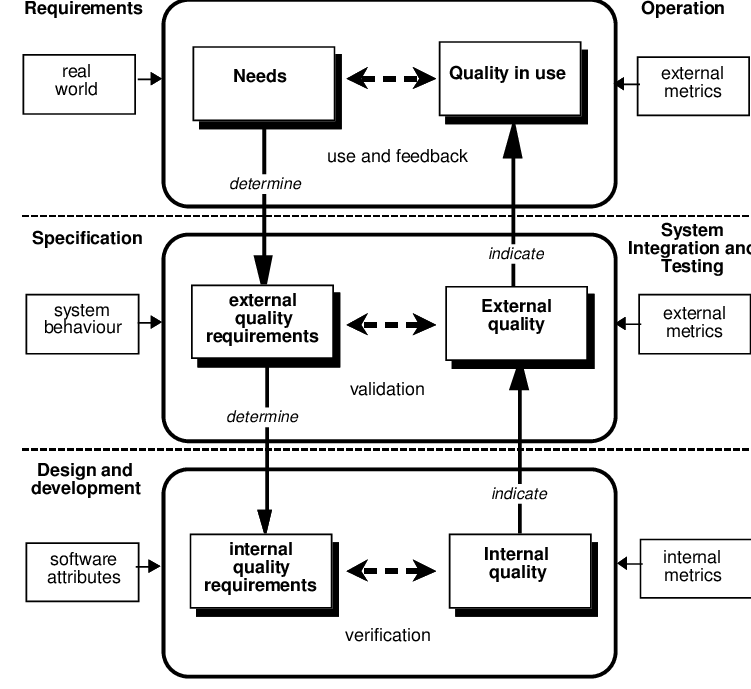
\includegraphics[width=0.7\textwidth]{../../assets/qualityVmodel.png}
    \caption{Modello a V}
    \label{fig:vmodel}
\end{figure}

Di seguito vengono indicate le metriche utilizzate per valutare la qualità del
prodotto e dei processi di sviluppo.

\subsection{Qualità di Processo} \label{qualita_processo}
In questa sezione vengono definite le metriche utilizzate per valutare
l'efficienza e l'efficacia dei processi del ciclo di vita del software, in
conformità con lo standard ISO/IEC 12207.

\subsubsection{Processi primari}

\paragraph{Processo di fornitura}

\metricdef{MPC-1}{Earned Value (EV)}{Valore del lavoro effettivamente completato in un determinato momento, espresso in termini di budget approvato.}
\metricformula{EV = \sum_{i} ( \% \text{Completamento}_i \times \text{Budget}_i )}

\metricdef{MPC-2}{Planned Value (PV)}{Valore del lavoro che si era pianificato di completare entro una certa data.}
\metricformula{PV = \sum_{i} (\% \text{Pianificato}_i \times \text{Budget}_i)}

\metricdef{MPC-3}{Actual Cost (AC)}{Costo realmente sostenuto per il lavoro svolto fino alla data corrente.}
\metricformula{AC = \sum \text{Costi Sostenuti}}

\metricdef{MPC-4}{Cost Performance Index (CPI)}{Indice di efficienza dei costi. Un valore $< 1$ indica che il progetto è fuori budget.}
\metricformula{CPI = \frac{EV}{AC}}

\metricdef{MPC-5}{Schedule Performance Index (SPI)}{Indice di efficienza della pianificazione. Un valore $< 1$ indica che il progetto è in ritardo.}
\metricformula{SPI = \frac{EV}{PV}}

\metricdef{MPC-6}{Estimate to Complete}{Rappresenta l'ammontare rimanente stimato per completare il progetto}
\metricformula{ETC = EAC-AC}

\metricdef{MPC-7}{Estimate at Completion (EAC)}{Stima totale dei costi alla fine del progetto, basata sulle performance attuali.}
\metricformula{EAC = \frac{BAC}{CPI}}

\paragraph{Processo di Sviluppo}

\metricdef{MPC-8}{Deployment Frequency}{Frequenza con cui il team rilascia nuove versioni del software, potenzialmente trasportabili in produzione.}
\metricformula{DF = \frac{\text{Numero di deployment}}{\text{Periodo di tempo}}}

\metricdef{MPC-9}{Requirements Stability Index}{Rappresenta la stabilità dei requisiti del prodotto software nel tempo.}
\metricformula{RSI = \frac{\#\text{Req originali} - (\#\text{Req modificati} + \#\text{Req eliminati} + \#\text{Req aggiunti})}{\#\text{Req originali}} \cdot 100}

\metricdef{MPC-10}{Average Build Time}{Tempo medio impiegato per completare il processo di build e test automatici.}
\metricformula{T_{avg} = \frac{\sum_{i=1}^{n} T_{build\_i}}{n}}

\paragraph{Processo di Documentazione}

\metricdef{MPC-11}{Indice di Gulpease}{Indice che valuta la leggibilità di un testo in lingua italiana. Valori bassi indicano bassa leggibilità.}
\metricformula{G = 89 + \frac{300 \times (\#\text{Frasi}) - 10 \times (\#\text{Lettere})}{\#\text{Parole}}}

\metricdef{MPC-12}{Correttezza Ortografica}{Misura la densità di errori ortografici presenti nella documentazione.}
\metricformula{C = \#\text{errori ortografici}}

\paragraph{Processo di Verifica}

\metricdef{MPC-13}{Code review turnaround time}{Tempo medio impiegato per completare una revisione del codice in vista di una Pull Request.}
\metricformula{CRT = \frac{\sum_{i=1}^{n} T_{review\_i}}{n}} $T_{review\_i}$ tempo impiegato per completare la revisione della PR $i$.

\metricdef{MPC-14}{Test success rate}{Percentuale di test superati rispetto al totale dei test eseguiti.}
\metricformula{TSR = \left( \frac{\#\text{Test superati}}{\#\text{Test eseguiti}} \right) \times 100}

\metricdef{MPC-15}{Code Coverage}{Percentuale di codice coperta da test}
\metricformula{CC = \frac{\#\text{LOC testate}}{\#\text{LOC totali}} \times 100}

\subsubsection{Processi Organizzativi}

\paragraph{Processo di Gestione dei Rischi} \label{gestione_rischi_operativi}

\metricdef{MPC-16}{Rischi non previsti}{Numero di rischi non previsti ad inizio periodo, per ciascun periodo di progetto.}
\metricformula{RNP_i = \#\text{Rischi non previsti nel periodo } i}

\paragraph{Processo di Gestione della qualità}

\metricdef{MPC-17}{Metriche soddisfatte}{Percentuale di metriche di qualità che vengono soddisfatte in un determinato istante di tempo.}
\metricformula{MS = \left( \frac{\#\text{Metriche soddisfatte}}{\#\text{Metriche totali}} \right) \times 100}

\subsection{Qualità di Prodotto} \label{qualita_prodotto}
In questa sezione vengono definite le metriche per valutare la qualità
intrinseca del prodotto software, basandosi sul modello ISO/IEC 9126.

\subsubsection{Funzionalità}

\metricdef{MPD-1}{Requisiti obbligatori soddisfatti}{Percentuale di requisiti funzionali obbligatori implementati e testati.}
\metricformula{R\textsubscript{ob} = \left( \frac{\text{Requisiti obbligatori soddisfatti}}{\text{Requisiti obbligatori totali}} \right) \times 100}

\metricdef{MPD-2}{Requisiti opzionali soddisfatti}{Percentuale di requisiti funzionali opzionali implementati e testati.}
\metricformula{R\textsubscript{op} = \left( \frac{\text{Requisiti opzionali soddisfatti}}{\text{Requisiti opzionali totali}} \right) \times 100}

\metricdef{MPD-3}{Requisiti desiderabili soddisfatti}{Percentuale di requisiti funzionali desiderabili implementati e testati.}
\metricformula{R\textsubscript{de} = \left( \frac{\text{Requisiti desiderabili soddisfatti}}{\text{Requisiti desiderabili totali}} \right) \times 100}

\subsubsection{Affidabilità}

\metricdef{MPD-4}{Broken links}{Numero di riferimenti ipertestuali all'interno dell'applicazione che non portano alla risorsa corretta o non portano ad alcuna risorsa.}
\metricformula{BL = \#\text{Broken Links}}

\metricdef{MPD-5}{Branch Coverage}{Percentuale di rami decisionali (if, switch, loop) percorsi durante i test.}
\metricformula{BC = \left( \frac{\text{Rami testati}}{\text{Rami totali}} \right) \times 100}

\metricdef{MPD-6}{Statement Coverage}{Percentuale di istruzioni (statements) del codice sorgente eseguite durante i test automatici.}
\metricformula{SC = \left( \frac{\text{Istruzioni testate}}{\text{Istruzioni totali}} \right) \times 100}

\subsubsection{Usabilità}

\metricdef{MPD-7}{Profondità di Navigazione}{Numero massimo di click necessari per raggiungere una qualsiasi pagina di contenuto partendo dalla vista principale.}
\metricformula{\max_{i \in I} \text{Click}_i \quad \begin{array}{l} (\text{dove } I = \text{insieme delle pagine}) \\ (\text{dove } \text{Click}_i = \text{numero di click per raggiungere la pagina } i) \end{array}}

\subsubsection{Efficienza}

\metricdef{MPD-8}{Indexing time}{Tempo di \glossario{indicizzazione} per un DiP di dimensioni standard (1-4GB).}
\metricformula{IT = \text{Tempo di indicizzazione (secondi)}}

\metricdef{MPD-9}{Search Time}{Tempo medio di risposta per un set di query predefinite.}
\metricformula{ST = \sum_{i=1}^{n} \frac{\text{Tempo di risposta}_i}{n} \quad \begin{array}{l} (\text{dove } n = \text{numero di query}) \\ (\text{dove }i = \text{indice della query}) \end{array}}

\metricdef{MPD-10}{Average CPU usage}{Percentuale media di utilizzo della CPU durante l'esecuzione del software. Si considera un campione di misurazioni effettuate in condizioni di carico (durante l'indicizzazione o la ricerca) nonché in idle. Quest'ultimo per assicurare che il software non consumi risorse inutilmente quando non è in uso.}
\metricformula{CPU_{avg} = \sum_{i=1}^{n} \frac{\text{Utilizzo CPU}_i}{n} \quad (\text{dove }n = \text{numero di misurazioni})}

\metricdef{MPD-11}{Peak memory usage}{Massima quantità di memoria RAM utilizzata durante l'esecuzione del software. Permette di individuare eventuale scarsa gestione delle risorse.}
\metricformula{MEM_{peak} = \max(\text{Utilizzo RAM}_i) \quad (\text{dove }i = 1, \dots, n, \text{istante di tempo } i)}

\subsubsection{Manutenibilità}

\metricdef{MPD-12}{Complessità Ciclomatica}{Misura la complessità del flusso di controllo del codice. Valori superiori a 15 indicano codice difficile da testare e manutenere.}
\metricformula{M = E - N + 2P \quad (\text{dove } E=\text{archi}, N=\text{nodi}, P=\text{componenti connessi})}

\metricdef{MPD-13}{Accoppiamento tra Classi (CBO)}{Numero di classi a cui una determinata classe è accoppiata (usa o è usata da). Un valore alto indica scarsa modularità.}
\metricformula{CBO = \frac{\#\text{Dipendenze}}{\#\text{Componenti}}}

\metricdef{MPD-14}{Code smells}{Numero di code smells, misurato ogni 1000 righe di codice (KLOC). I code smells sono indicatori di potenziali problemi di design o implementazione.}

\subsubsection{Portabilità}

\metricdef{MPD-15}{SO Compatibility}{Numero di sistemi operativi supportati dal software. Un valore alto indica una maggiore portabilità.}
\metricformula{SO_{comp} = \#\text{Sistemi operativi supportati}}

\subsection{Strumenti}
\subsubsection{Jira Software}
Utilizzato come strumento di Project Management per il tracciamento dei
requisiti e la gestione del workflow.
\begin{itemize}
    \item \textbf{Metriche associate:} MPC-1 \dots MPC-7 (Earned Value Management), MPC-17 (Metriche soddisfatte), MPD-1 \dots MPD-3 (Requisiti).
    \item \textbf{Utilizzo:} Attraverso la funzione di esportazione \glossario{JQL} $\rightarrow$ csv, e uno script python appositamente sviluppato, vengono estratti i dati necessari per il calcolo delle metriche di Earned Value e dei requisiti soddisfatti, permettendo un monitoraggio costante dell'andamento del progetto.
\end{itemize}

\subsubsection{GitHub \& GitHub Actions}
Viene utilizzato per il controllo di versione e l'automazione della CI/CD.
\begin{itemize}
    \item \textbf{Metriche associate:} MPC-8 (Deployment Frequency), MPC-10 (Avg Build Time), MPC-13 (Code Review Turnaround Time), MPC-14 (Test success rate).
    \item \textbf{Utilizzo:} I workflow di GitHub Actions oltre che garantire la metrica MPC-14 (Test success rate) attraverso l'esecuzione di test automatici, permettono di tracciare i tempi di build e code review, fornendo dati utili per il calcolo delle metriche di processo.
\end{itemize}

\subsubsection{Strumenti di Analisi Statica e Qualità del Codice}

\paragraph{SonarQube}
Piattaforma centrale per la \textit{Continuous Inspection} del codice
TypeScript (Angular) e JavaScript (Electron).
\begin{itemize}
    \item \textbf{Metriche associate:} MPD-6 (Statement Coverage), MPD-5 (Branch Coverage), MPD-12 (Complessità Ciclomatica), MPD-13 (CBO), MPD-14 (Code Smells).
    \item \textbf{Utilizzo:} Analizza staticamente il codice ad ogni \glossario{Push}, verificando che il superamento dei \glossario{Quality Gates} stabiliti sia coerente con le soglie definite nelle metriche di manutenibilità.
\end{itemize}

\paragraph{Aspell \& Script Python (Custom)}
Data la natura della documentazione in lingua italiana, si rende necessario uno
strumento specifico per l'analisi testuale.
\begin{itemize}
    \item \textbf{Metriche associate:} MPC-11 (Indice di Gulpease), MPC-12 (Correttezza Ortografica).
    \item \textbf{Utilizzo:} Uno script Python che utilizza la libreria \texttt{textstat} per il calcolo dell'indice di Gulpease e le API di \textit{Aspell} per il conteggio degli errori ortografici nei file Markdown/\glossario{LaTeX}.
\end{itemize}

\subsubsection{Strumenti di Testing e Performance (Electron-Angular)}

\paragraph{Playwright}
Framework di testing End-to-End utilizzato per simulare l'interazione utente
all'interno dell'ambiente Electron.
\begin{itemize}
    \item \textbf{Metriche associate:} MPD-7 (Profondità di Navigazione).
    \item \textbf{Utilizzo:} Viene configurato un \glossario{crawler} automatizzato che percorre l'albero di navigazione dell'applicazione Angular, validando la raggiungibilità dei link e calcolando il numero di interazioni (click) necessarie per raggiungere i nodi foglia.
\end{itemize}

\paragraph{Electron Manager \& Chrome DevTools Protocol}
Per misurare l'efficienza di un'applicazione Electron, è necessario monitorare
l'istanza di Chromium sottostante.
\begin{itemize}
    \item \textbf{Metriche associate:} MPD-10 (Average CPU usage), MPD-11 (Peak memory usage).
    \item \textbf{Utilizzo:} Durante le sessioni di test automatizzati con Playwright, vengono invocati script Node.js che interrogano le API \texttt{process.getProcessMemoryInfo()} e \texttt{process.getCPUUsage()} di Electron per campionare il consumo di risorse in idle e sotto carico.
\end{itemize}

\paragraph{TotalValidator}
Integrato nei tool di sviluppo, viene utilizzato per profilare i tempi di
risposta dell'interfaccia Angular.
\begin{itemize}
    \item \textbf{Metriche associate:} MPD-4 (Broken links).
    \item \textbf{Utilizzo:} Controllo formale di consistenza e correttezza della struttura dell'interfaccia utente Angular.
\end{itemize}

\paragraph{Funzioni interne di misurazione performance}
Integrate direttamente nel codice sorgente, queste funzioni permettono di
misurare i tempi di indicizzazione e risposta alle query, fornendo dati precisi
per le metriche MPD-8 (Indexing time) e MPD-9 (Search Time).

\vfill
\begin{flushright}
    \textit{7-ZPUs}
\end{flushright}

\end{document}